%http://cms-results.web.cern.ch/cms-results/public-results/preliminary-results/SUS-16-024/index.html

%% CVSId: $Id: Example.tex,v 1.1.1.1 2000/11/28 11:15:12 exupery Exp $
\documentclass[%
xcolor=dvipsnames,table%,pdftex%,
%pdf,
%nocolorBG,
%colorBG,
%slideColor,
%slideBW,
%draft,
%frames
%azure
%contemporain
%nuancegris
%troispoints
%lignesbleues
%darkblue
%alienglow
%autumn
%12pt
]{beamer}
%%%%%%%%%%%%%%%%%%%%%%%%%%%%%
%\mode<presentation>
%{
  %\usetheme{Madrid}
 \usetheme[progressbar=frametitle]{metropolis}% \usetheme{Boadilla}
  % or ...
%%%%%%%%%%%%%%%%%%%%%%%%%%%%%%%%%%%%%
%para revelar texto a aparecer en overlays
  %\setbeamercovered{transparent} 
  %\setbeamercovered{invisible}
%%%%%%%%%%%%%%%%%%%%%%%%%%%%%%%%%%%%%
  % \setbeamertemplate{blocks}[rounded][shadow=true]
  % \setbeamertemplate{navigation symbols}{}

  % \setbeamertemplate{footline}{%\hspace*{.5cm}
  %   \scriptsize{\phantom{Gg}%\insertauthor 
  %     \hspace*{50pt} 
  %     \hfill \insertframenumber
  %     \hspace*{.5cm}}}

  % % or whatever (possibly just delete it)
  % %\useoutertheme{shadow} 
  % \setbeamercolor{postit}{fg=black,bg=yellow}
  % \setbeamercolor{white}{fg=black,bg=white}
  % \setbeamercolor{cite}{fg=black,bg=yellow}
%}


\usepackage[absolute,overlay]{textpos}
\usepackage{booktabs}
\usepackage[scale=2]{ccicons}

%\usepackage{pgfplots}
%\usepgfplotslibrary{dateplot}

%%%%%%%%%%%%%%%%%%%%%%%%%%%%%%
%Force pdflatex processing even with "$ latex" (required by arXiv)
%\pdfoutput=1
\graphicspath{{figures/}}
%\usepackage[T1]{fontenc}
%\usepackage[utf8]{inputenc}
%\usepackage[spanish]{babel}
%\spanishdecimal{.}
%\usepackage{marvosym}
%\usepackage{beamerprosper}
\usepackage{amsmath,amssymb}
\usepackage{overpic}
\usepackage{graphicx}
\usepackage{mycolors}
%\usepackage{xmpmulti}
\usepackage{multimedia}
\usepackage{pgf}
\usepackage{cancel}
\usepackage{wasysym}
%\usepackage{helvet}
\usepackage{comment}
\usepackage{array}   % for \newcolumntype macro
\newcolumntype{L}{>{$}l<{$}} % math-mode version of "l" column type
\includecomment{comentar}
\specialcomment{comentar}
{\begingroup}{\medskip\endgroup}
\excludecomment{comentar}

\includecomment{comentario}
\specialcomment{comentario}
{\begingroup}{\endgroup}
\excludecomment{comentario}

\includecomment{details}
\specialcomment{details}
{\begingroup}{\endgroup}
\excludecomment{details}

%\usepackage[texcoord,grid,gridunit=mm,gridcolor=red!10,subgridcolor=green!10]{eso-pic}


\newcommand{\widescreen}{
\setlength{\paperwidth}{171 mm}
\setlength{\paperheight}{96 mm}
\setlength{\textwidth}{151 mm}
\setlength{\textheight}{86 mm}
}

 \widescreen


\title{Dark matter in left-right symmetric standard model}
\subtitle{triplet scalar dark matter portal  }


%\subtitle
%{Reconstruction of the neutrino mass matrix} % (optional)

\author{Diego Restrepo}
% - Use the \inst{?} command only if the authors have different
%   affiliation.
\institute{
  \begin{columns}
    \begin{column}{0.4\textwidth}
Instituto de F\'\i sica\\
Universidad de Antioquia\\
Phenomenology Group\\
\url{http://gfif.udea.edu.co}      
    \end{column}
    \begin{column}{0.5\textwidth}
      \hfill 5th Uniandes Particle Physics School\\
      \hfill 
\includegraphics[scale=0.25]{ua}\\
      %\hfill \tiny{Image credits}
    \end{column}
  \end{columns}
\quad\\
\quad\\
{\tiny
\alert{\textbf{Focus on}} \\
arXiv:1703.08148 (PRD)\\
\alert{In collaboration with}\\
  C.~Arbeláez (UFSM)\& M.~Hirsch (IFIC)}
%\centering
}
% - Use the \inst command only if there are several affiliations.
% - Keep it simple, no one is interested in your street address.

\date{\tiny May 21, 2017 } % (optional) \today
%{
\includegraphics[scale=0.3]{udea}}
\titlegraphic{\hfill
\includegraphics[height=1.5cm]{udea}}

%\subject{Talks}
% This is only inserted into the PDF information catalog. Can be left
% out. 



% If you have a file called "university-logo-filename.xxx", where xxx
% is a graphic format that can be processed by latex or pdflatex,
% resp., then you can add a logo as follows:

% \pgfdeclareimage[height=0.5cm]{university-logo}{university-logo-filename}
% \logo{\pgfuseimage{university-logo}}



% Delete this, if you do not want the table of contents to pop up at
% the beginning of each subsection:
%\AtBeginSubsection[]
%{
%  \begin{frame}<beamer>
%    \frametitle{Outline}
%    \tableofcontents[currentsection,currentsubsection]
%  \end{frame}
%}

\newcommand{\chml}[2]{$\underline{\text{#1\hspace{#2}}}$}
\begin{document}


%===============
\begin{comentar}
%===============  
%=============
\end{comentar}
%=============

\maketitle

\begin{frame}
  \frametitle{Table of Contents}
% %\small
% %\vspace{-0.5cm}
   \setbeamertemplate{section in toc}[sections numbered]
   \tableofcontents[hideallsubsections]
\end{frame}

%\section{Motivation}

\section{Review of SM}
\begin{frame}
  \frametitle{Only fields}
  Lorentz\invisible<1>{+$U(1)$}:
  \begin{align}
    \mathcal{L}=\only<1>{-\tfrac{1}{4}\left( \partial^{\mu} A^{\nu}-\partial^{\nu} A^{\mu} \right) \left( \partial_{\mu} A_{\nu}-\partial_{\nu} A_{\mu} \right) \,.  }
\only<2>{\partial_{\mu}\phi^{\color{red}*}\partial^{\mu}\phi-{\color{red}m^2} \phi^{\color{red}*}\phi-\lambda \left( \phi^{\color{red}*}\phi \right)^2\,.}
  \end{align}
  \begin{align*}
   A^\mu(x)\to {A'}^\mu(x)=&{\Lambda^\mu}_\nu A^\nu(\Lambda^{-1}x)&&\text{Vector field}\nonumber\\
   \phi(x)\to \phi'(x)=&\phi(\Lambda^{-1} x) && \text{Scalar field}\nonumber\\
    \psi_\alpha(x)\to\psi'_\alpha(x)=&{\left[ S(\Lambda) \right]_\alpha}^\beta\psi_\beta(\Lambda^{-1}x)\,, &&\text{Left Weyl spinor}\nonumber\\
\left(  \psi_\alpha(x) \right)^{\dagger}=\psi_{\dot{\alpha}}^{\dagger}(x)\to{\psi'}_{\dot{\alpha}}^{\dagger}(x)=&{\left[ S^*(\Lambda)\right]_{\dot{\alpha}}}^{\dot{\beta}} \psi_{\dot{\beta}}^{\dagger}(\Lambda^{-1}x)\,,&&\text{Right anti-Weyl spinor}
\end{align*}
With
\begin{align*}
  S(\Lambda)=
\exp\left( \boldsymbol{\xi}\cdot \frac{\boldsymbol{\sigma}}{2}+i\boldsymbol{\theta}\cdot \frac{\boldsymbol{\sigma}}{2} \right)\,,
\end{align*}
where $\boldsymbol{\sigma}=(\sigma_1,\sigma_2,\sigma_3)$ are the Pauli matrices. $\overline{\boldsymbol{\sigma}}\equiv-\boldsymbol{\sigma}$.

\end{frame}

\begin{frame}
  \frametitle{Weyl spinor}
  \begin{align}
  \mathcal{L}=&i{\psi}^{\dagger}_{\dot{\alpha}}\overline{\sigma}^{\mu \dot{\alpha}\alpha}\partial_\mu\psi_{\alpha}-
m \left( \psi^{\alpha}\psi_{\alpha}+\psi^{\dagger}_{\dot{\alpha}}\psi^{\dagger \dot{\alpha}} \right) \nonumber\\
=&i{\psi}^{\dagger}\overline{\sigma}^\mu\partial_\mu\psi-
m \left( \psi\psi+\psi^{\dagger}\psi^{\dagger} \right)\,.
\end{align}


\end{frame}

\begin{frame}
  \frametitle{Electron field: \emph{one in four}: Dreiner,... arXiv:0812.1594 (PR)}
\vspace{-0.7cm}

\begin{align*}
\text{Scalar product:}\qquad  {{}^{\alpha}}\,{}_{\alpha}\qquad \text{and}\qquad {{}_{\dot{\alpha}}}\,{}^{\dot{\alpha}}\,.
\end{align*}
\rowcolors{1}{RoyalBlue!20}{}
    \begin{tabular}{llll}
    Name \hspace{4cm} & Symbol Name \hspace{1.5cm} & Lorentz Name \hspace{1.5cm} & $U(1)$\\\hline
    $e_L$: left electron  & $\xi_{\alpha}$ & ${\left[ S \right]_{\alpha}}^{\beta}$ & $e^{i\theta}$\\
   $\left( e_L \right)^{\dagger}=e^{\dagger}_R$: right positron    & $\left( \xi_{\alpha} \right)^{\dagger}=\xi^{\dagger}_{\dot{\alpha}}$ & ${\left[{S^{*}}\right]_{\dot{\alpha}}}^{\dot{\beta}}$ & $e^{-i\theta}$\\
   $e_R$: right electron    & $\left( \eta^{\alpha} \right)^{\dagger}=\eta^{\dagger\;\dot{\alpha}}$ & ${\left[ \left( S^{-1} \right)^\dagger \right]^{\dot{\alpha}}}_{\dot{\beta}}$& $e^{i\theta}$\\
   $\left( e_R \right)^{\dagger}=e^{\dagger}_L$: left positron&$\eta^{\alpha}$& ${\left[ \left( S^{-1} \right)^T \right]^{\alpha}}_{\beta}$ & $e^{-i\theta}$\\\hline
  \end{tabular}

\begin{align*}
  \mathcal{L}=&i\xi^{\dagger}_{\dot{\alpha}}\overline{\sigma}^{\mu\;\dot{\alpha}\alpha}\partial_{\mu}\xi_{\alpha}+i\eta^{\alpha}\sigma^{\mu}_{\alpha\dot{\alpha}}\partial_{\mu}\eta^{\dagger\;\dot{\alpha}}
-m \left(\eta^{\alpha} \xi_{\alpha}+\xi^{\dagger}_{\dot{\alpha}} \eta^{\dagger\;\dot{\alpha}}\right)\nonumber\\
=&i\xi^{\dagger}\overline{\sigma}^{\mu}\partial_{\mu}\xi+i\eta\sigma^{\mu}\partial_{\mu}\eta^{\dagger}
-m \left(\eta\xi+\xi^{\dagger}\eta^{\dagger} \right)+\,.
\end{align*}
\centering

\includegraphics[scale=0.13]{counting-1-to-4}
\end{frame}


\section{Dark matter}

\begin{frame}
\begin{picture}(320,250)
\only<1>{\put(-24,-22){\begin{overpic}[scale=0.352]{z2}\end{overpic}}}%
\end{picture}
\end{frame}

\begin{frame}
\begin{picture}(320,250)
\only<1->{\put(-24,-22){\begin{overpic}[scale=0.352]{z2_bkg}\end{overpic}}}%
\only<1->{\put(250,180){\begin{overpic}[scale=0.25]{brickY}\end{overpic}}}%
\only<1->{\put(220,110){\begin{overpic}[scale=0.25]{brickR}\end{overpic}}}%
\only<1->{\put(350,110){\begin{overpic}[scale=0.25]{brickB}\end{overpic}}}%
\only<1->{\put(120,20){\begin{overpic}[scale=0.25]{brickssY}\end{overpic}}}%
\only<1->{\put(220,20){\begin{overpic}[scale=0.25]{brickssR}\end{overpic}}}%
\only<1->{\put(350,20){\begin{overpic}[scale=0.25]{brickssB}\end{overpic}}}%
\end{picture}
\end{frame}









\begin{frame}
  \frametitle{Dark matter}
\rowcolors{1}{RoyalBlue!20}{}
   \begin{tabular}{llllll}
 $\text{Name}$ & $\text{Symbol}$ & $\text{SU}(3)_c$ & $\text{SU}(2)_L $& $\text{U}(1)_Y$ & $Z_2$ \\ \hline
 $\begin{pmatrix}\nu_L  &  e_L\end{pmatrix}^{\operatorname{T}}$ & $
\begin{pmatrix}\xi_{1\alpha}  &  \xi_{2\alpha} \end{pmatrix}^{\operatorname{T}}$ & $ \mathbf{1} $ & $ \mathbf{2} $ & $ -1/2 $ & $ +1$\\
$(e_R)^{\dagger} $ & $ \eta^{\alpha}_1 $ & $ \mathbf{1} $ & $ \mathbf{1} $ & $ +1 $ & $ +1$ \\
$(\psi_R)^{\dagger} $ & $ \eta^{\alpha}_2 $ & $ \mathbf{1} $ & $ \mathbf{1} $ & $ +1 $ & $ -1$ \\
$\psi_L $ & $ \xi_{3\alpha} $ & $ \mathbf{1} $ & $ \mathbf{1} $ & $ -1 $ & $ -1$ \\
$S$ &  & $ \mathbf{1} $ & $ \mathbf{1} $ & $ 0 $ & $ -1$ \\
 \end{tabular}

 \begin{align}
   \mathcal{L}=& M_{\psi} \left[ \left( \psi_R \right)^{\dagger} \psi_L
\left( \psi_L \right)^{\dagger} \psi_R \right]
+ h_S \left[ S \left(e_R  \right)^{\dagger} \psi_L 
+ S \left( \psi_L \right)^{\dagger}e_R 
\right]
 \end{align}
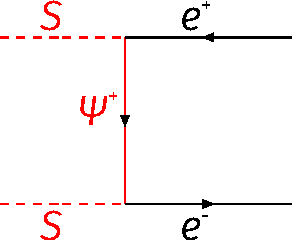
\includegraphics[scale=0.5]{fp}

\end{frame}


\end{document}

\section{SARAH}

\begin{frame}
  \frametitle{Version control}
\begin{picture}(320,250)
\only<1>{\put(-10,20){
  \begin{overpic}[scale=0.5]{ss1}
  \end{overpic}
}}%
\only<2>{\put(-10,20){
  \begin{overpic}[scale=0.5]{ss2}
  \end{overpic}
}}
\end{picture}


\end{frame}

\section{Reproducibility }
\begin{frame}
\begin{picture}(320,250)
\only<1>{\put(-30,-20){\begin{overpic}[scale=0.51]{sssfdm1}\end{overpic}}}%
\only<2>{\put(-30,-20){\begin{overpic}[scale=0.51]{sssfdm2}\end{overpic}}}%
\only<3>{\put(-30,-20){\begin{overpic}[scale=0.51]{sssfdm3}\end{overpic}}}%
\only<4>{\put(-30,-20){\begin{overpic}[scale=0.51]{sssfdm4}\end{overpic}}}%
\only<5>{\put(-30,-20){\begin{overpic}[scale=0.51]{sssfdm5}\end{overpic}}}%
\only<6>{\put(-30,-20){\begin{overpic}[scale=0.51]{sssfdm6}\end{overpic}}}%
\only<7>{\put(-30,-20){\begin{overpic}[scale=0.51]{sssfdm7}\end{overpic}}}%
\only<8>{\put(-30,-20){\begin{overpic}[scale=0.51]{sssfdm8}\end{overpic}}}%
\only<9>{\put(-30,-20){\begin{overpic}[scale=0.51]{sssfdm9}\end{overpic}}}%
\end{picture}
\end{frame}



\begin{frame}
  \frametitle{Unification: $SO(10)$}
  \begin{columns}
    \begin{column}{0.7\textwidth}
      \begin{small}
  \begin{align*}
    \mathbf{16}_{F_{i}}=
    \begin{pmatrix}
      {{\color{green}u_{R}}^{\dagger}}\\
      {{\color{blue}u_{R}}^{\dagger}}\\
      {{\color{red}u_{R}}^{\dagger}}\\
      {{\color{green}u_{L}}}\\
      {{\color{blue}u_{L}}}\\
      {{\color{red}u_{L}}}\\
      {{\color{green}d_{L}}}\\
      {{\color{blue}d_{L}}}\\
      {{\color{red}d_{L}}}\\
      {{\color{green}d_{R}}^{\dagger}}\\
      {{\color{blue}d_{R}}^{\dagger}}\\
      {{\color{red}d_{R}}^{\dagger}}\\
      \nu_L\\
      e_L\\
      {e_{R}}^{\dagger}\\
      N\\
    \end{pmatrix}_{i} \qquad\Rightarrow \mathcal{L}_{SM}\supset h\, \mathbf{16}_F\times\mathbf{16}_{F}\times \mathbf{10}_{S}+\text{h.c}
  \end{align*}
      \end{small}
    \end{column}
    \begin{column}{0.3\textwidth}
  \hfill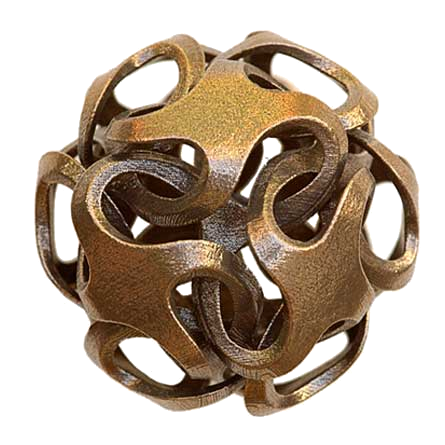
\includegraphics[scale=0.2]{sym}      
    \end{column}
  \end{columns}


\end{frame}


\begin{frame}
\frametitle{Not-susy $\operatorname{SO}(10)\to SU(5)\to \operatorname{SU}(3)_C\times SU(2)_L \times \operatorname{U}(1)_Y \times Z_2 $}
\begin{picture}(320,250)
%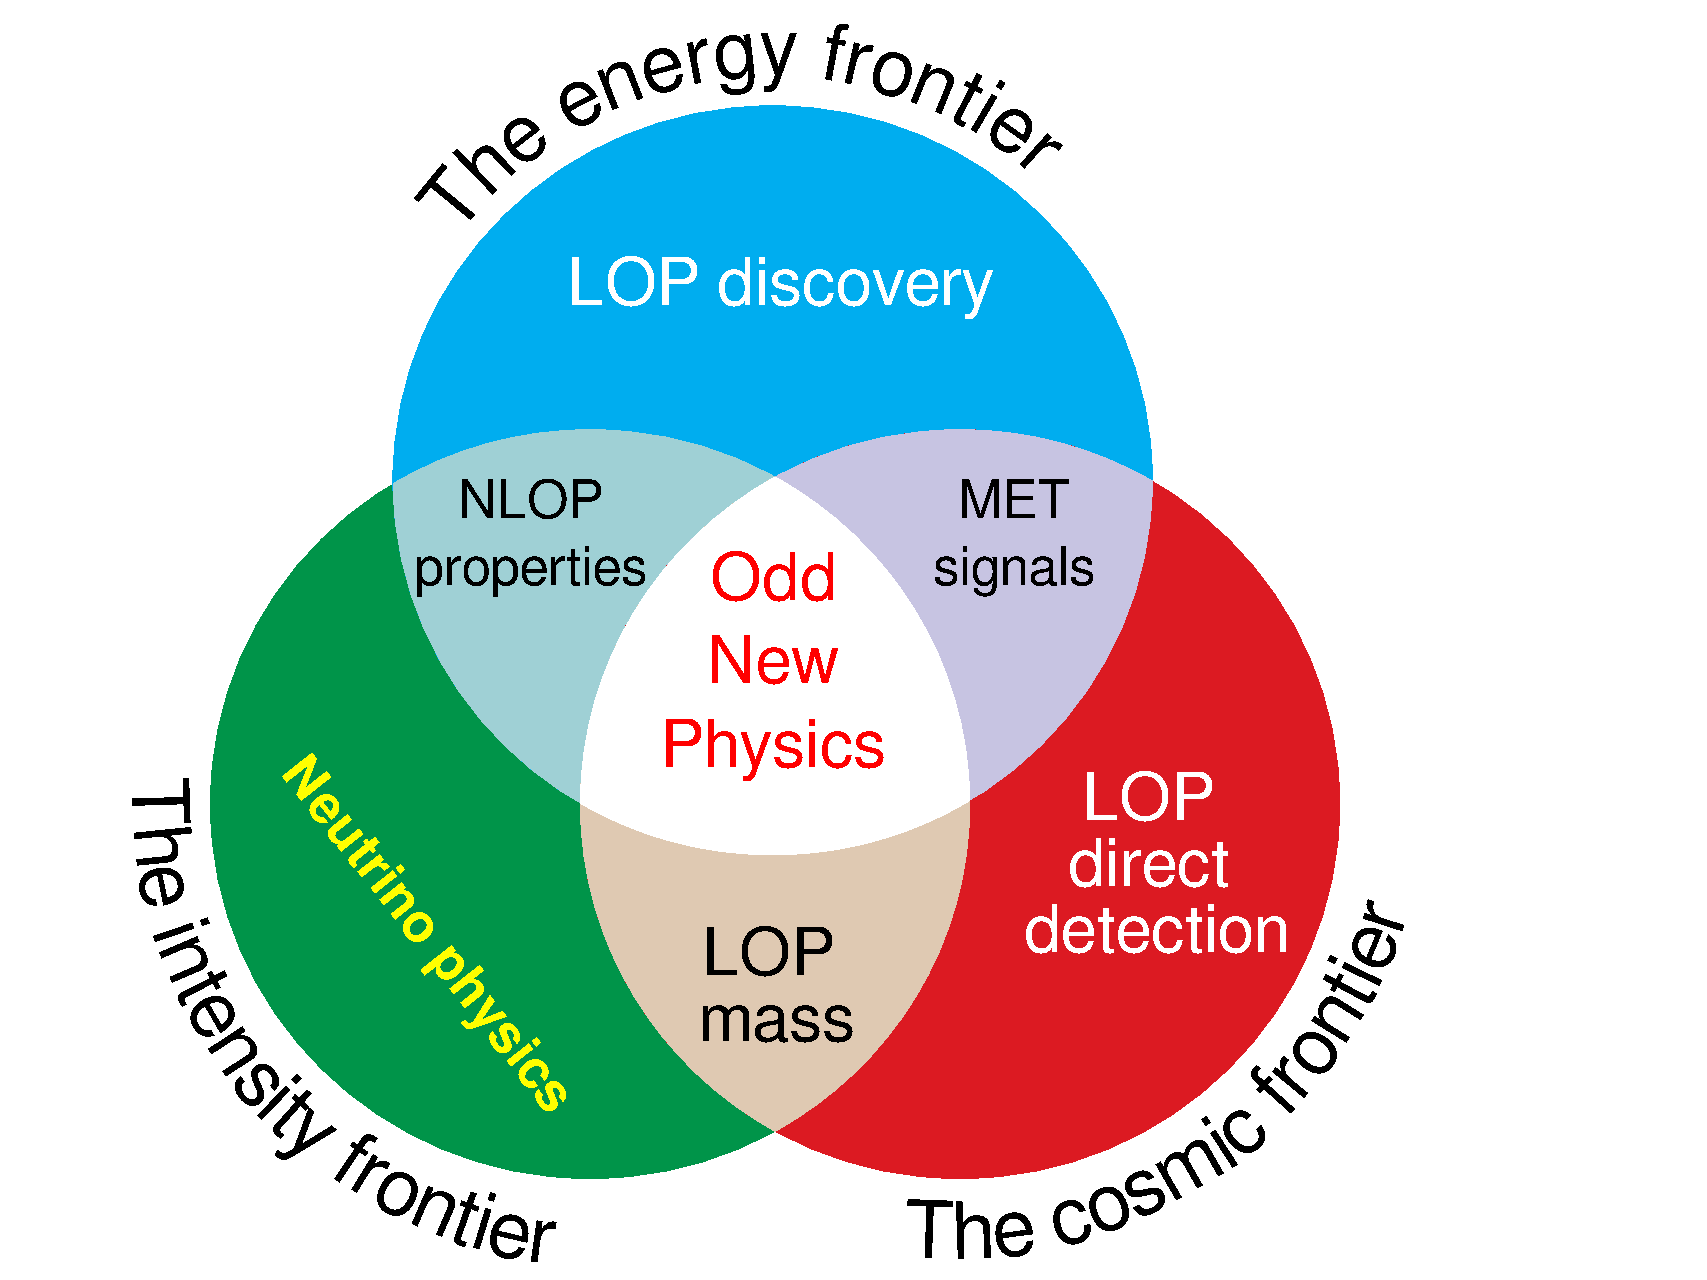
\includegraphics[scale=0.2]{tocrs}
 %   
 % \only<1->{\put(-11,10){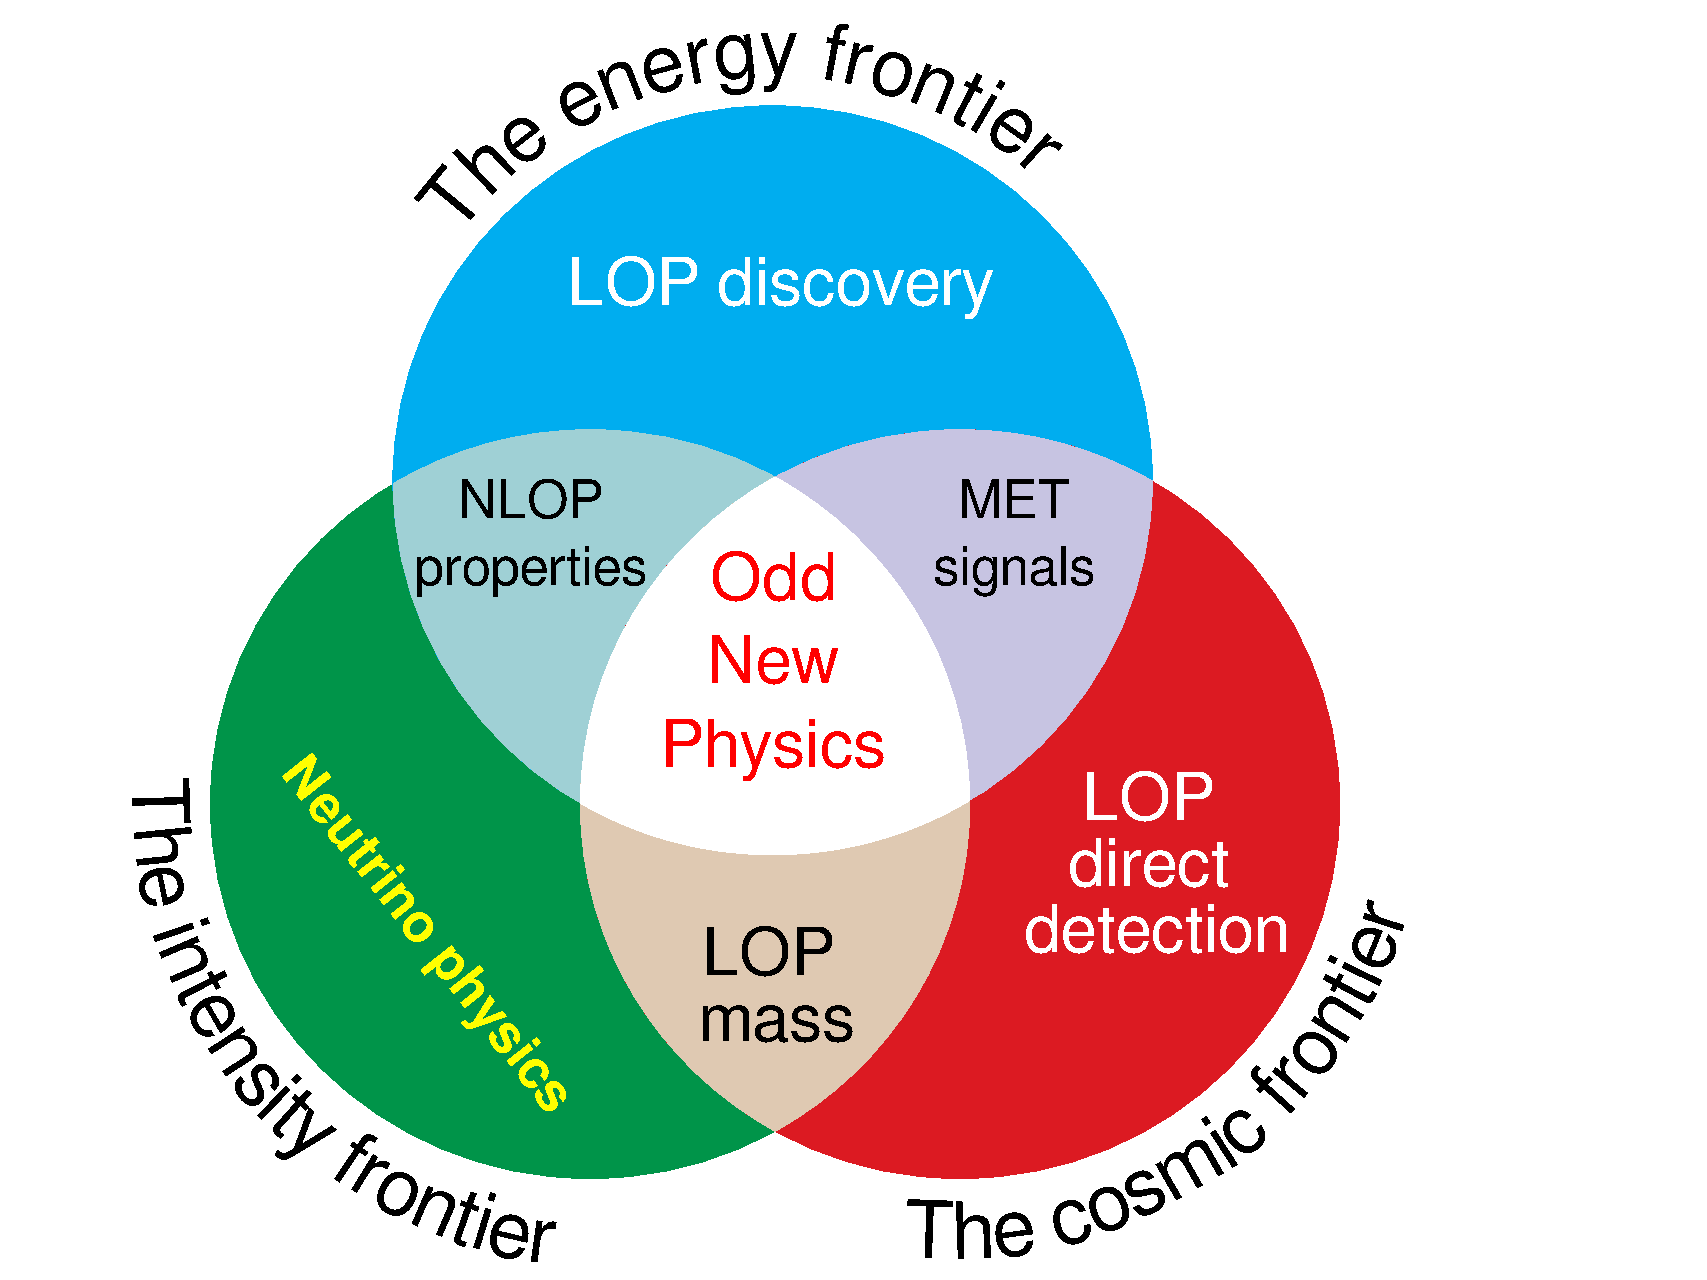
\includegraphics[scale=0.4]{tocrs}}}%
 % 
 \only<1->{\put(-10,250){
  \begin{columns}[T,onlytextwidth]
    \column{0.5\textwidth}
      \metroset{block=fill}
      \begin{block}{Standard Model: $Z_2$-even }
        Fermions: $\boldsymbol{16}_F$

        Scalars: $\boldsymbol{10}_H,\boldsymbol{45}_H\cdots$
      \end{block}


    \column{0.5\textwidth}

      \metroset{block=fill}


      \begin{alertblock}{New $Z_2$-odd particles}
       \color{red}
        $\boldsymbol{10}_F,\boldsymbol{45}_F,\cdots$
       
        $\boldsymbol{16}_H,\cdots$
      \end{alertblock}
  \end{columns}
}
}
\only<1->{\put(-10,190){
    \begin{minipage}[t]{1.0\textwidth}
 \alert{Lightest Odd Particle (LOP)} may be  a suitable dark matter candidate, \alert{and can improve gauge coupling unification }
    \end{minipage}
}
}
\only<1>{\put(0,10){
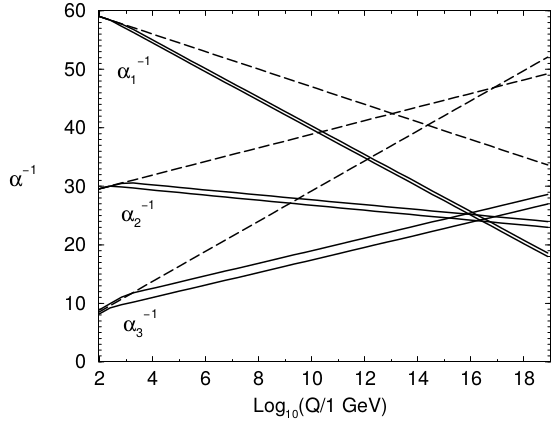
\includegraphics[scale=0.45]{smunif}
}
}
\only<2->{\put(0,80){
  \begin{overpic}[height=3cm%,grid
            ]{table1}
\put(16,0){\tikz \draw[red,thick,rounded corners,fill=orange,fill opacity=0.2] (0,0) rectangle (0.5,0.5);}
\put(62,0){\tikz \draw[red,thick,rounded corners,fill=orange,fill opacity=0.2] (0,0) rectangle (0.5,0.5);}
\put(38,-7){\tikz \draw[red,thick,rounded corners,fill=orange,fill opacity=0.2] (0,0) rectangle (1.,0.5);}
\only<5>{\put(18,-7){\tikz \draw[red,thick,rounded corners,fill=orange,fill opacity=0.2] (0,0) rectangle (0.9,0.5);}}
\only<3->{\put(16,6){\tikz \draw[green,thick,rounded corners,fill=green,fill opacity=0.2] (0,0) rectangle (1.,0.5);}}
\only<3->{\put(50,6){\tikz \draw[green,thick,rounded corners,fill=green,fill opacity=0.2] (0,0) rectangle (0.5,0.5);}}
\only<3-4>{\put(16,13){\tikz \draw[blue,thick,rounded corners,fill=blue,fill opacity=0.2] (0,0) rectangle (0.5,0.5);}}
\only<3-4>{\put(55,13){\tikz \draw[blue,thick,rounded corners,fill=blue,fill opacity=0.2] (0,0) rectangle (0.5,0.5);}}
\only<5>{\put(16,13){\tikz \draw[orange,thick,rounded corners,fill=orange,fill opacity=0.2] (0,0) rectangle (0.5,0.5);}}
\only<4->{\put(30,5){\tikz \draw[black,thick,rounded corners,fill=black,fill opacity=0.2] (0,0) rectangle (1.,0.6);}}
\only<4->{\put(32,8){\parbox[t]{2cm}{$\mathbf{2}_{1/2}^{S}$}}}
  \end{overpic}
  \begin{overpic}[height=3cm%,grid
            ]{table2}
\only<4->{\put(30,30){\tikz \draw[black,thick,rounded corners,fill=black,fill opacity=0.2] (0,0) rectangle (0.5,0.5);}}
  \end{overpic}
}
}
\only<2-5>{\put(0,70){
  \begin{minipage}[t]{1.0\linewidth}
    $SU(3)_{C}: \mathbf{3}\; (T),\ \mathbf{6},\ \mathbf{8}\;(\Lambda) $
  \end{minipage}
}
%\put(40,38){\color{red}${}^{2}$}
}
\only<2>{\put(0,70){
  \begin{minipage}[t]{1.0\linewidth}
    \begin{align*}
      m_{3_0}=2.7\ \text{TeV},\qquad m_{\Lambda}\sim 10^{10}\ \text{TeV},\qquad m_{\text{GUT}}\sim 10^{16}\ \text{GeV}\,.
    \end{align*}
    arXiv:0912.1545 (Frigerio-Hambye) %check for second doublet
  \end{minipage}
}
}
\only<3>{\put(0,70){
  \begin{minipage}[t]{1.0\linewidth}
\centering
     \alert{Split-SUSY like}

    %uniftwo451E16
    arXiv:1509.06313 (C. Arbelaez, R. Longas, D.R, O. Zapata)
  \end{minipage}
}
}
%%%circle
\invisible<1-3>{\put(125,90){      \metroset{block=fill}
    \begin{minipage}[t]{0.68\linewidth}
      \begin{exampleblock}{\only<4>{Radiative hybrid seesaw (Parida {%\tiny 
1106.4137}) or} 1509.06313}
      \centering
 \tiny
      \only<4>{Partial  Split-}SUSY-like spectrum: {\color{red}bino}-higgsino-{\color{red}wino}

               \hfill             + $\color{red}\hspace{3cm}\downarrow$\hspace{3cm}    
        
         $\boldsymbol{10}'_H$ with fermion DM or, \hspace{0.5cm}  \color{red}
         $\boldsymbol{16}_H,\cdots$ with scalar DM 
        
      \end{exampleblock}
    \end{minipage}
}
}
\end{picture}
\end{frame}

%%%%
\begin{frame}
  \frametitle{Dilepton plus transverse missing energy signal}
\vspace{-0.3cm}
  \begin{center}
    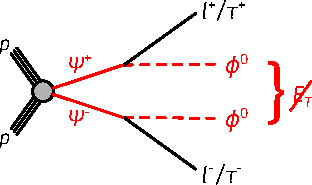
\includegraphics[scale=1]{fig_02ai}

\vspace{-0.2cm}

    $\operatorname{SU}(2)_L$ assignments:

\vspace{-0.8cm}
  \begin{align*}
    \color{red}
    \Psi=&\color{red}\boldsymbol{1},\boldsymbol{2} (\Psi),\boldsymbol{3} (\Sigma)\,,&\color{red}\Phi\color{red}=&\color{red}\boldsymbol{1},\boldsymbol{2}\,,\ \text{with}\ m_{\text{DM}}\sim m_{h}/2\,.
  \end{align*}
\vspace{-1.3cm}

\hrulefill

\vspace{-0.4cm}

Simplified SUSY models
  \end{center}
\vspace{-0.8cm}
  \begin{overpic}[scale=0.9%,grid
            ]{fig_02a}
    \put(26,48){$\color{red}\tilde{l}/$}    
    \put(26,23){$\color{red}\tilde{l}/$}    
    \put(73,70){$l/$}    
    \put(73,2){$l/$}    
    \put(-15,-10){Smaller cross sections.}    
  \end{overpic}\hfill
  \begin{overpic}[scale=0.9%,grid
            ]{fig_02b}
    \put(-70,-10){Intermediate states and smaller lepton $\cancel{\boldsymbol{p}_{\text{T}}}$}
    %\only<2>{\put(-180,180){\hspace{1cm}\color{blue} Benchmark point: 100 GeV \hspace{1cm}60 GeV }}    
  \end{overpic}
\end{frame}
% * <restrepo@udea.edu.co> 2015-11-15T12:45:09.589Z:
%
% Explanation of the framework
%
% ^.

\begin{frame}
\frametitle{$m_{\phi^{0}}=60\ \text{GeV}$ }
\hspace{-1.4cm}\begin{overpic}[scale=0.7]{emuMVA}  
%%
%\includegraphics
\end{overpic}

Full analysis on flavor space: 
F. von der Pahlen, G. Palacio, DR, O. Zapata arXiv:1605.01129 [PRD] 
\end{frame}



\begin{frame}
  \frametitle{{\color{red}Singlet-Doublet}-Triplet fermion dark-matter}
The most general $\text{SO}(10)$ invariant Lagrangian contains the following Yukawa terms
\begin{align*}
-\mathcal{L} & \supset  Y{\bf 10}_F {\bf 45}_F {\bf 10}_H + M_{\mathbf{45}_F}{\bf 45}_F{\bf 45}_F + M_{\mathbf{10}_F}{\bf 10}_F{\bf 10}_F
\invisible<1-3>{+{\mathcal{L}(\alert{\mathbf{10}_\Phi}\invisible<4>{\ \text{or}\   \mathbf{16}_\Phi})}.} 
\end{align*}



  \begin{columns}
    \begin{column}{0.47\textwidth}
Basis $\boldsymbol{\psi}^0=\left({\color{red}N},\Sigma^0,{\color{red}\psi_L^0},{\color{red}\left( \psi_R^0 \right)^{\dagger}}\right)^T$ 
\tiny
\begin{align*}
  &\mathcal{M}_{\boldsymbol{\psi}^0}=\nonumber\\
&\begin{pmatrix}
{\color{red}M_N}          &   0       &{\color{red}-y\,c_\beta v/\sqrt{2}}&{\color{red}y\,s_\beta v/\sqrt{2}} \\
0 & M_\Sigma &  f\,c_{\beta'}v/\sqrt{2} & -f\,s_{\beta'}v/\sqrt{2}\\
{\color{red}-y\,c_\beta} v/\sqrt{2} &  f\,c_{\beta'}v/\sqrt{2}  & 0            & {\color{red}}-M_D\\
{\color{red}y\,s_\beta v/\sqrt{2}}& -f\,s_{\beta'}v/\sqrt{2}&{\color{red}}  -M_D                &  0  \\
\end{pmatrix},
\end{align*}
    \end{column}
    \begin{column}{0.53\textwidth}
      %\only<2>{
\includegraphics[scale=0.38]{rumor}}
      \invisible<1>{%
      \only<1-2>{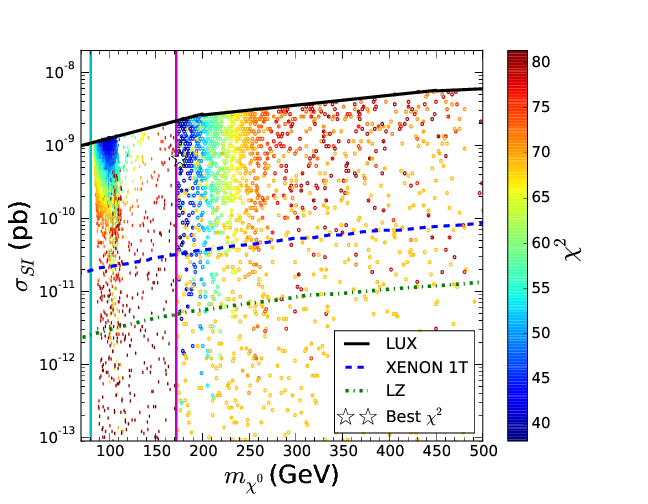
\includegraphics[scale=0.35]{GCE}}\only<3>{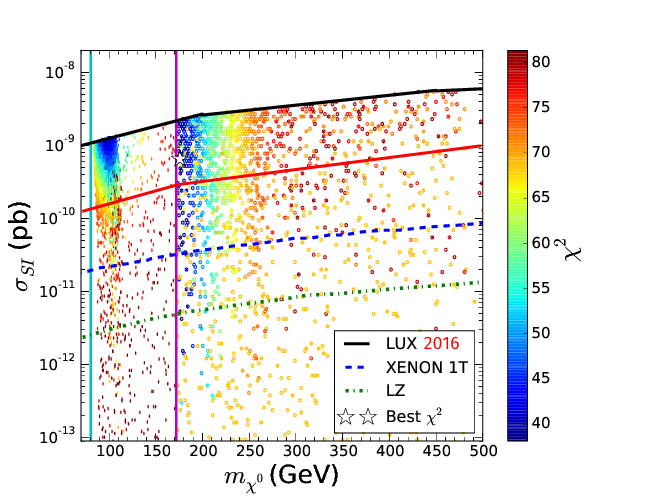
\includegraphics[scale=0.35]{GCE2016}}%
      \only<4>{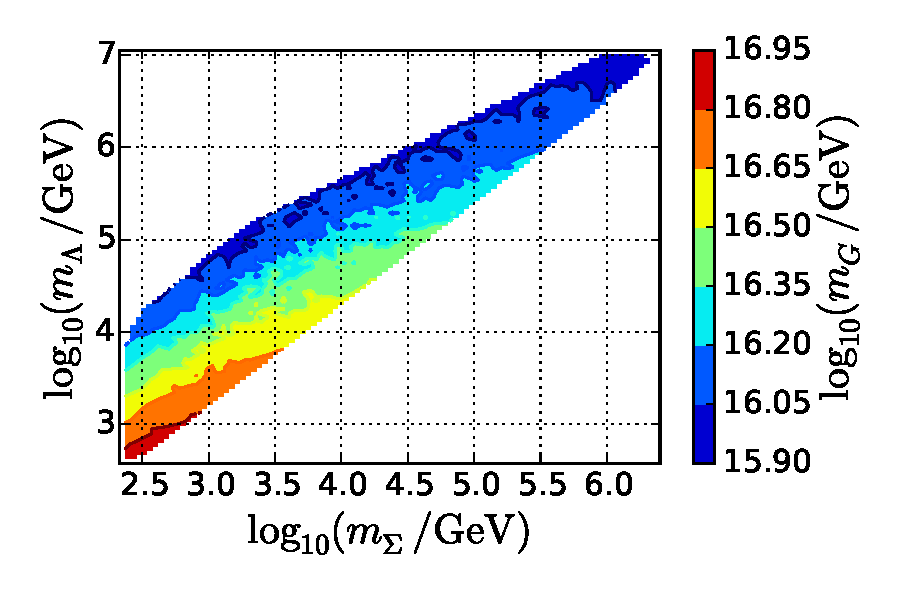
\includegraphics[scale=0.43]{uniftwo451E16}} 
      }%
    \invisible<1>{\only<1-3>{\tiny  \quad \\ S. Horiuchi, O. Macias, DR, A. Rivera, O. Zapata, 1602.04788 (JCAP)}%
                 \only<4>{\tiny \quad \\ Split-SUSY:  like $\alert{M_{\Phi}}=2\ \text{TeV}$}%
                 }
    \end{column}
  \end{columns}

\vspace{-1.5cm}
%  \invisible<2->
{ $\mathbf{10}_F \to \psi_L,\left( \psi_R \right)^{\dagger}$\\
                  $\mathbf{45}_F \to \Sigma,\Lambda$\\
                  $\mathbf{45}'_F \to N$\\
\invisible<2->{arXiv:1511.06495: signals at 100 TeV collider}
%Model used in: arXiv:1511.06495\\
%{\small \textbf{Physics Opportunities of a 100 TeV Proton-Proton Collider}\\
%Nima Arkani-Hamed, T. Han, M. Mangano, LT Wang. }
}
\end{frame}


\begin{frame}
  \frametitle{Is the glass half empty or half full?}
   Tree-level SM-portal could be fully excluded in the near future

  \begin{columns}
    \begin{column}{0.5\textwidth}
      \begin{itemize}
      \item Singlet scalar dark matter
      \item Inert doublet model
      \item Tree-level SM-portal dark matter $\cdots$
      \end{itemize}
    \end{column}
    \begin{column}{0.5\textwidth}

      \only<1>{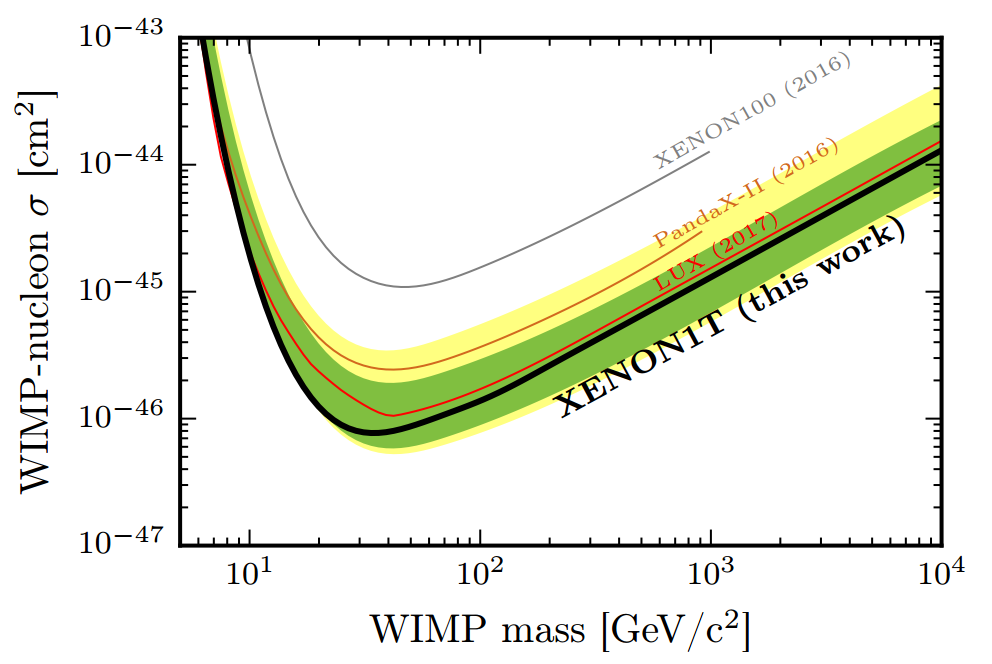
\includegraphics[scale=0.2]{x1t} }%
      \only<2->{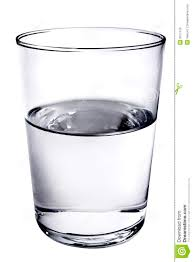
\includegraphics[scale=0.3,angle=180]{halffill} }

    %\hfill  \tiny{\url{Dreamstime.com}}  
    \end{column}

  \end{columns}

  In this talk we explore
  \begin{itemize}
  \item<2-> Recover SM-portals in LR models 
  \item<3-> New portals in LR models 
  \end{itemize}

\end{frame}




\section{Left-Right symmetric realization}

\begin{frame}
  \frametitle{Singlet-doublet fermion dark matter}

\begin{table}[t]
\rowcolors{1}{RoyalBlue!20}{}
\begin{tabular}{c|c|c|c|c}
{Field} & Multiplicity & $3_{c}2_{L}2_{R}1_{B-L}$& Spin & $\text{SO}(10)$ origin\\
\hline
$\Phi$ & 1 & $(1,2,2,0)$ & 0& $10$\\
$\chi$, $\chi^{c}$ & 1 & $(1,2,2,0)$ %$\oplus (1,2,1,-1)$ 
 & 1/2& $10$\\
 $N$  & 1 & $(1,1,1,0)$& 1/2& 45\\
\end{tabular}
\caption{The relevant part of the field content. Note that, the two fermion doublets $\chi$ and $\chi^{c}$ come from an only fermionic LR bidoublet. In the third column the relevant fields are
characterized by their $\text{SU}(3)_{c}\times \text{SU}(2)_{L}\times
\text{SU}(2)_{R}\times \text{U}(1)_{B-L}$ quantum numbers while their $\text{SO}(10)$
origin is specified in the fourth column. }
\label{tab:ModelI}
\end{table}
\end{frame}

\begin{frame}
  \frametitle{Unification}
  \begin{table}%[h]
\small
\rowcolors{1}{RoyalBlue!20}{}
\begin{tabular}{c|c|c}
 $m_{\text{LR}} \,(\mbox{GeV})$ &  $3_{c}2_{L}2_{R}1_{B-L}$  & $m_{G}\,(\mbox{GeV})$ \\ \hline

 {$2\times 10^{3}$ }  & ${\color{blue}\Phi_{1,2,2,0}+2\Phi_{1,1,3,-2}}+\alert{\Psi_{1,1,3,0}} + \Phi_{1,1,3,0}+\Phi_{8,1,1,0}$ & $1.65 \times 10^{16}$   \\
 
 $\vdots$ &  $\vdots$  & $\vdots$   \\ 
\end{tabular}
\caption{ $\color{blue}{\Delta_{L,R}}=2\Phi_{1,1,3,-2}$. $m_{\text{LR}}$ and $m_{G}$ are given in GeV.}
\label{tab:I}
\end{table}

\end{frame}

% \section{Connect with Enrico work}
% \begin{frame}
%   \frametitle{Asymmetric}
  
% \end{frame}

\section{Triplets}

\begin{frame}
  \frametitle{\only<1>{Minimal Left-Right Symmetric Standard Model}\only<2>{Left-singlet  right-triplet DM}}
  \begin{center}
    \rowcolors{1}{RoyalBlue!20}{}
      \begin{tabular}{c|c|c|c|c}
\hline
%From Slansky: See SO(10) -> SU(2)xSU(2)*SU(4) and SU(4)-> SU(3)xU(1)
{Field} & Multiplicity & $3_{c}2_{L}2_{R}1_{B-L}$& Spin & $\text{SO}(10)$ origin\\
\hline
$Q$ & 3 & $(3,2,1,+\tfrac{1}{3})$ & 1/2 &16\\
$Q^{c}$ & 3 & $(\bar 3,1,2,-\tfrac{1}{3})$ &1/2& 16\\
$L$  & 3 & $(1,2,1,-1)$& 1/2& 16\\
$L^{c}$& 3 & $(1,1,2,+1)$  & 1/2& 16\\
\hline
$\Phi$ & 1 & $(1,2,2,0)$ & 0& $10$\\
$\Delta_R$ & 1 & $(1,1,3,-2)$ & 0& $126$\\ %DEBUG: check
\hline 
\invisible<1>{%
$\Psi_{1130}$ & 1 & $(1,1,3,0)$ & 1/2& $45$\\
}%
\invisible<1-2>{%
$\Psi_{1132}$ & 1 & $(1,1,3,2)$ & 1/2& $126$\\
$\Psi_{113-2}$ & 1 & $(1,1,3,-2)$ & 1/2& $\overline{126}$\\
\hline 
}%
\invisible<1-2>{%
$\Psi_{1310}$ & 1 & $(1,3,1,0)$ & 1/2& $45$\\
$\Psi_{8110}$ & 1 & $(1,1,8,0)$ & 1/2& $45$\\
$\Psi_{321\frac{1}{3}}$ & 1 & $(3,2,1,1/3)$ & 1/2& $16$\\
$\Psi_{321-\frac{1}{3}}$ & 1 & $(1,2,3,-1/3)$ & 1/2& $\overline{16}$\\
\hline 
}%
\end{tabular}
  \end{center}
\invisible<2->{\phantom{aa}}
\end{frame}

\begin{frame}
  \frametitle{$\Omega h^{2} = 0.1199 \pm 0.0027$ at $3\sigma$}
  \begin{figure}
    \centering
    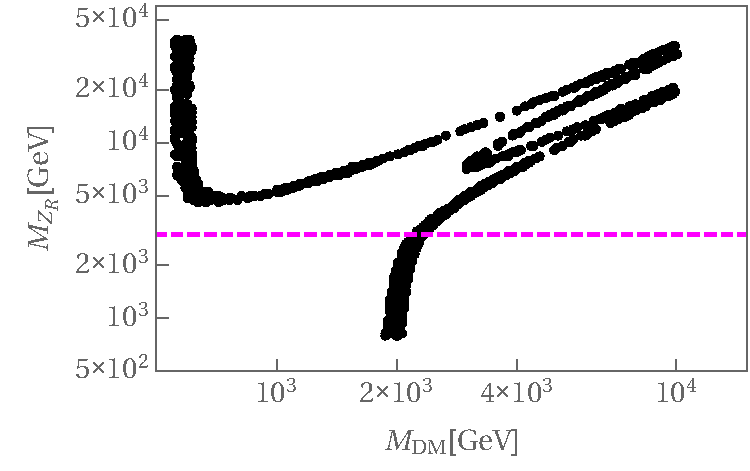
\includegraphics[scale=0.9]{Fig5}  %  
    \caption{Proper relic density scan: $0.5<v_R/\text{TeV}<50$}
  \end{figure}

   
\end{frame}

\begin{frame}
  \frametitle{Mixed Left-singlet right-triplet  DM}
  \begin{center}
    \rowcolors{1}{RoyalBlue!20}{}
      \begin{tabular}{c|c|c|c|c}
\hline
%From Slansky: See SO(10) -> SU(2)xSU(2)*SU(4) and SU(4)-> SU(3)xU(1)
{Field} & Multiplicity & $3_{c}2_{L}2_{R}1_{B-L}$& Spin & $\text{SO}(10)$ origin\\
\hline
$Q$ & 3 & $(3,2,1,+\tfrac{1}{3})$ & 1/2 &16\\
$Q^{c}$ & 3 & $(\bar 3,1,2,-\tfrac{1}{3})$ &1/2& 16\\
$L$  & 3 & $(1,2,1,-1)$& 1/2& 16\\
$L^{c}$& 3 & $(1,1,2,+1)$  & 1/2& 16\\
\hline
$\Phi$ & 1 & $(1,2,2,0)$ & 0& $10$\\
$\Delta_R$ & 1 & $(1,1,3,-2)$ & 0& $126$\\ %DEBUG: check
\hline 
\invisible<0>{%
$\Psi_{1130}$ & 1 & $(1,1,3,0)$ & 1/2& $45$\\
}%
\invisible<1>{%
$\Psi_{1132}$ & 1 & $(1,1,3,2)$ & 1/2& $126$\\
$\Psi_{113-2}$ & 1 & $(1,1,3,-2)$ & 1/2& $\overline{126}$\\
\hline 
}%
\invisible<1-2>{%
$\Psi_{1310}$ & 1 & $(1,3,1,0)$ & 1/2& $45$\\
$\Psi_{8110}$ & 1 & $(1,1,8,0)$ & 1/2& $45$\\
$\Psi_{321\frac{1}{3}}$ & 1 & $(3,2,1,1/3)$ & 1/2& $16$\\
$\Psi_{321-\frac{1}{3}}$ & 1 & $(1,2,3,-1/3)$ & 1/2& $\overline{16}$\\
\hline 
}%
\end{tabular}
  \end{center}
\invisible<2->{\phantom{aa}}
\end{frame}

\begin{frame}
  \frametitle{Setup}

\begin{equation}
\Psi_{1132} = 
 \begin{pmatrix}
  \Psi^{+}/\sqrt{2} & \Psi^{++}  \\
  \Psi^{0} & -\Psi^{+}/\sqrt{2} \\
 \end{pmatrix}, \hspace{0.8cm}
{\bar\Psi}_{113-2} = 
 \begin{pmatrix}
  \Psi^{-}/\sqrt{2} & \overline{\Psi}^{0}  \\
  \Psi^{--} & -\Psi^{-}/\sqrt{2} \\
 \end{pmatrix}.
\end{equation}


  \begin{align}
L\supset &\alert{M_{11}}\operatorname{Tr}(\Psi_{1130}\Psi_{1130})+\alert{M_{23}}\operatorname{Tr}(\Psi_{1132}{\bar\Psi}_{113-2})\nonumber\\
&+{\color{blue}\lambda_{13}}\operatorname{Tr}({\color{blue}\Delta_{R}}{\bar\Psi}_{113-2}\Psi_{1130})
+{\color{blue}\lambda_{12}}\operatorname{Tr}(\Delta^{\dagger}_{R}\Psi_{1132} \Psi_{1130})\, ,
\end{align}

\begin{align}
{\color{blue}\tan\gamma}=&\frac{\lambda_{13}}{\lambda_{12}}\,,& {\color{blue} \lambda}=&\sqrt{\lambda_{12}^2+\lambda_{13}^2}\,.
\end{align}

Blind spot at
\begin{align}
  M_{23}\sin2\gamma - M_{\text{DM}}=0
\end{align}

\end{frame}

\begin{frame}
  \frametitle{Proper relic density scan}
\def\fh{5cm}
\begin{figure}
  \centering
  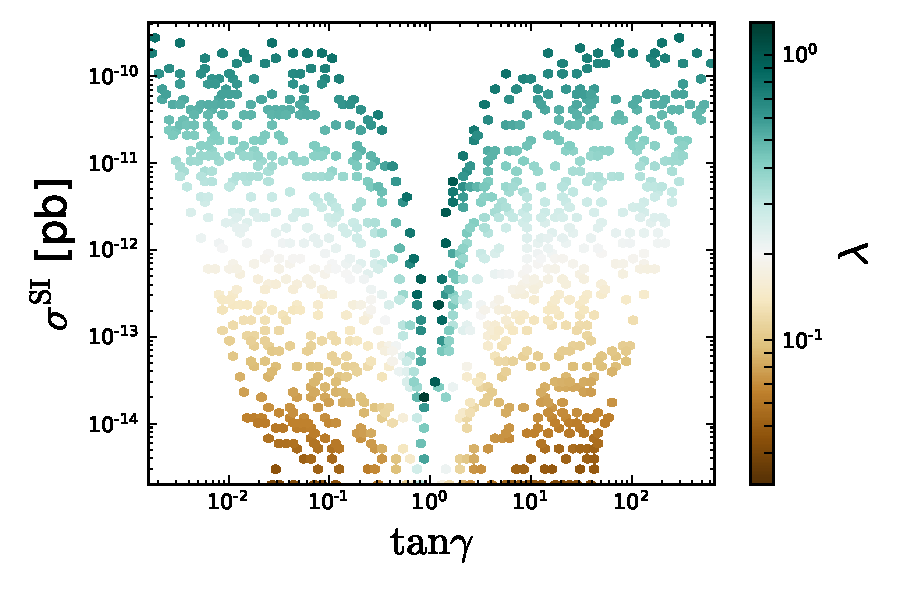
\includegraphics[height=\fh]{lambda}
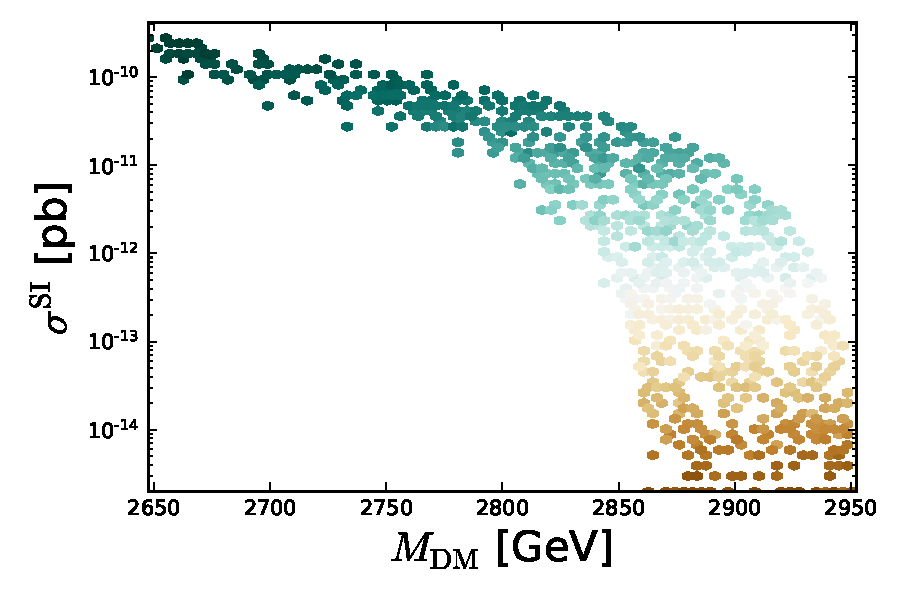
\includegraphics[height=\fh,width=4cm]{ssi_Mdm}
  \caption{$M_{11}=50\ \text{TeV}$ $2.7<M_{23}/\text{TeV}<3.1$ \qquad  (Right:  $\tan\gamma>5$)}
\end{figure}
\end{frame}

\begin{frame}
  \frametitle{$\Omega h^{2} = 0.1199 \pm 0.0027$ at $3\sigma$}
  \begin{figure}
    \centering
    \only<1>{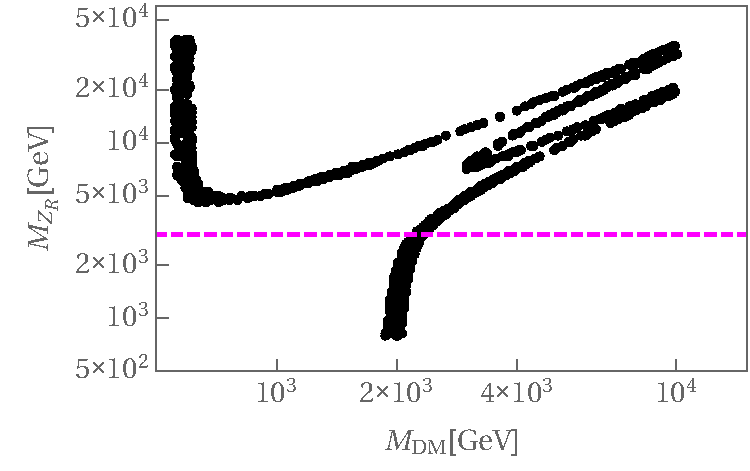
\includegraphics[scale=0.78]{Fig5}}%
    \only<2>{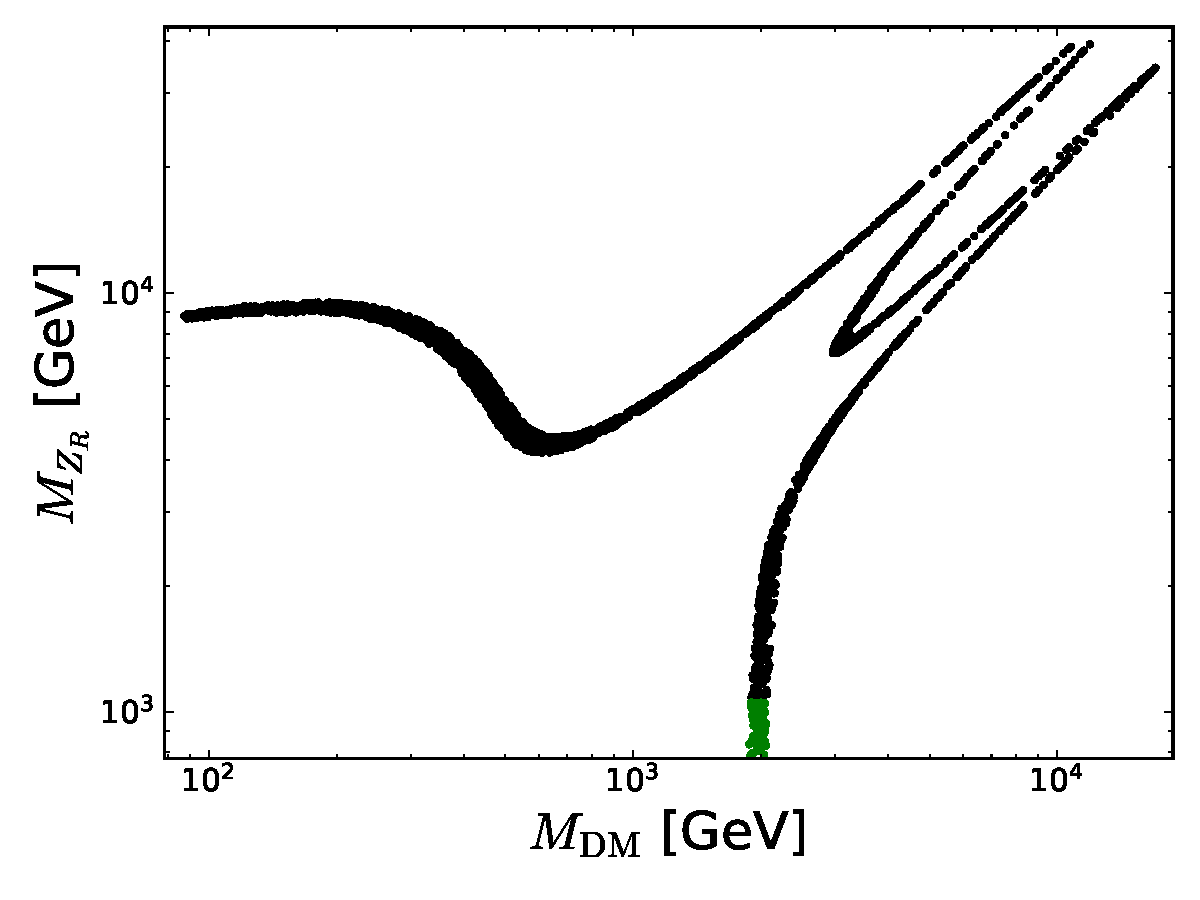
\includegraphics[width=0.55\textwidth]{IIMDMvsMZRExa5}}
    \caption{\invisible<1>{Proper relic density scan:  $v_{R}: [2, 50]$ TeV, $M_{23}:[0.2, 50]$ TeV, $M_{11}: 50$ TeV,  $\tan\gamma=-1$ and $\lambda=0.14$.}}
  \end{figure}

 \end{frame}
 \begin{frame}
    \frametitle{Direct detection cross section}
    \begin{figure}
      \centering
      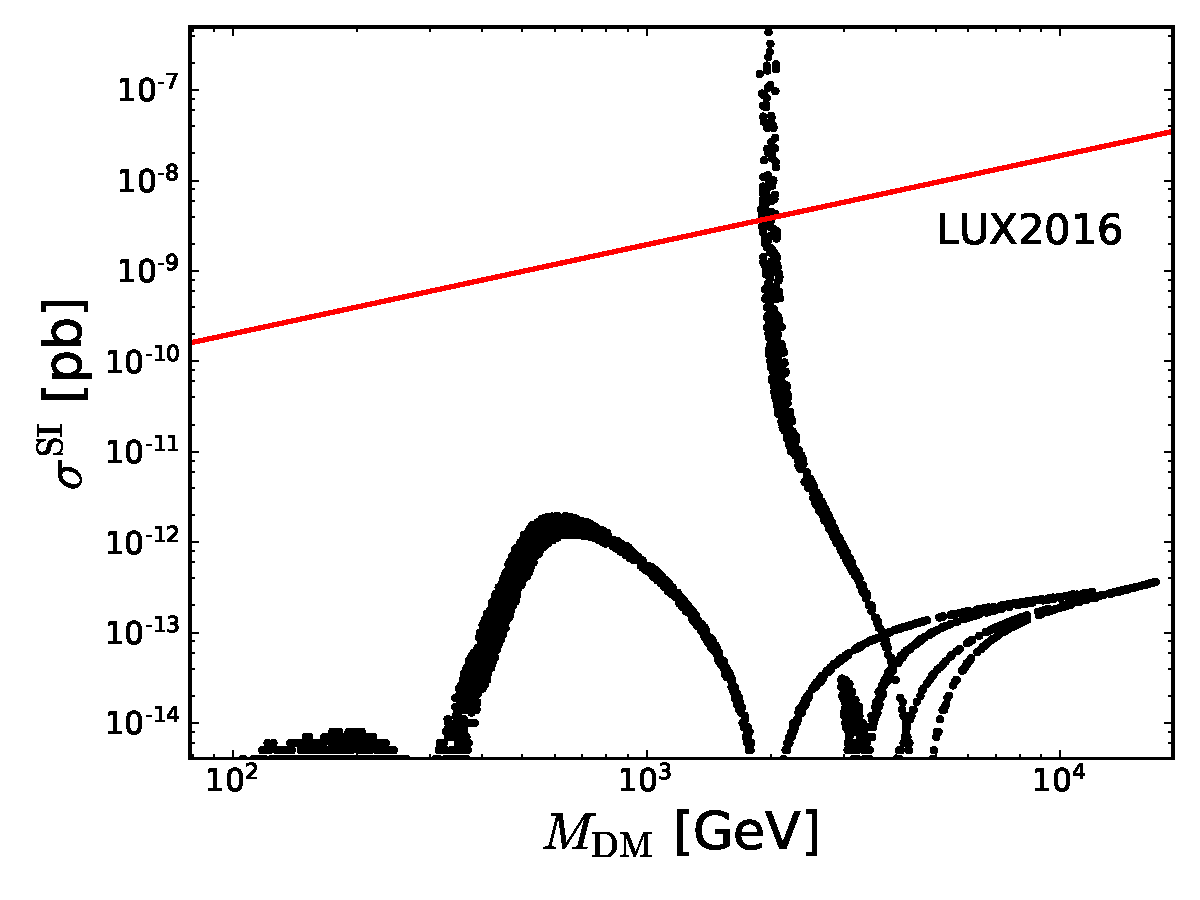
\includegraphics[width=0.53\textwidth]{MDMvsDDExa5} 
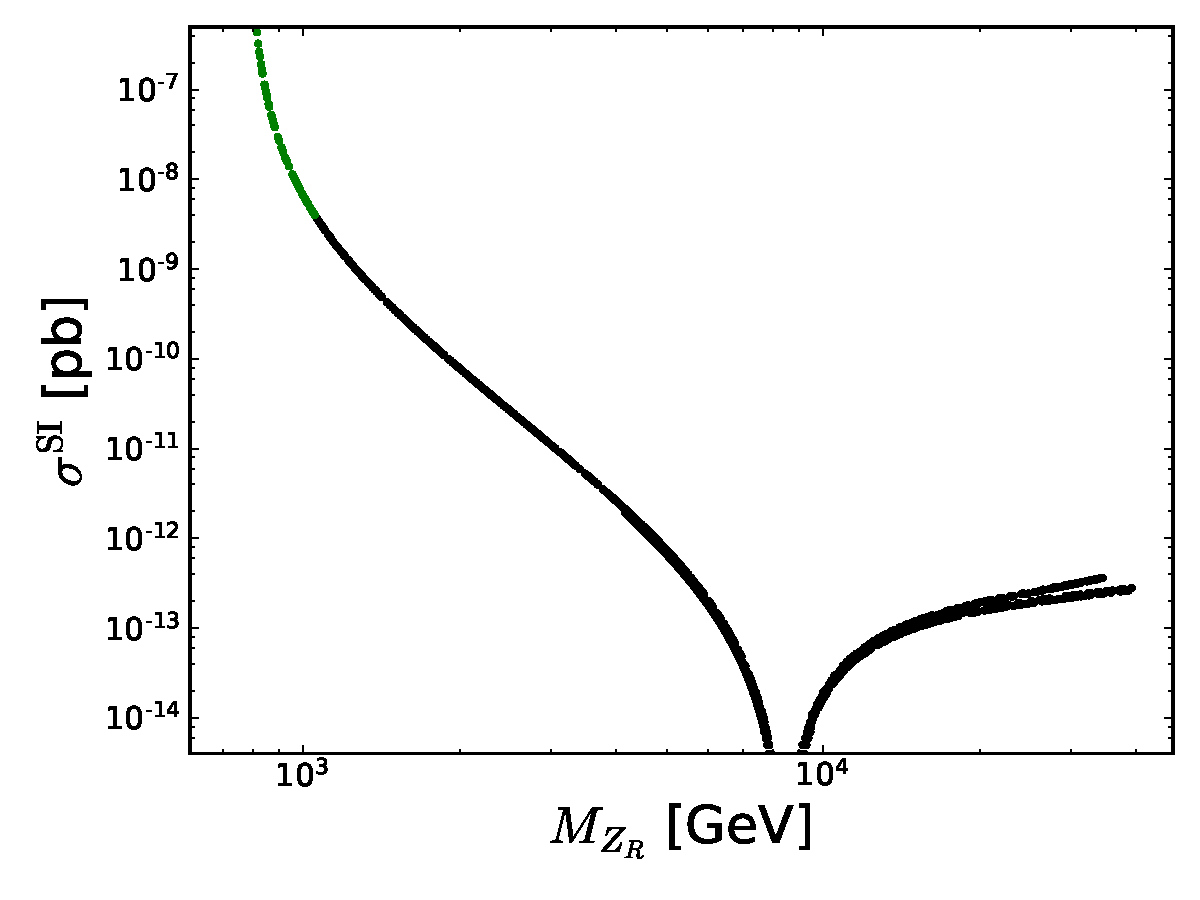
\includegraphics[width=0.53\textwidth]{IIMZRvsDDExa5} 
      \caption{ $v_{R}: [2, 50]$ TeV, $M_{23}:[0.2, 50]$ TeV, $M_{11}: 50$ TeV,  $\tan\gamma=-1$ and $\lambda=0.14$.}
    \end{figure}
\end{frame}


\begin{frame}
  \frametitle{Unification}
  \begin{center}
    \rowcolors{1}{RoyalBlue!20}{}
      \begin{tabular}{c|c|c|c|c}
\hline
%From Slansky: See SO(10) -> SU(2)xSU(2)*SU(4) and SU(4)-> SU(3)xU(1)
{Field} & Multiplicity & $3_{c}2_{L}2_{R}1_{B-L}$& Spin & $\text{SO}(10)$ origin\\
\hline
$Q$ & 3 & $(3,2,1,+\tfrac{1}{3})$ & 1/2 &16\\
$Q^{c}$ & 3 & $(\bar 3,1,2,-\tfrac{1}{3})$ &1/2& 16\\
$L$  & 3 & $(1,2,1,-1)$& 1/2& 16\\
$L^{c}$& 3 & $(1,1,2,+1)$  & 1/2& 16\\
\hline
$\Phi$ & 1 & $(1,2,2,0)$ & 0& $10$\\
$\Delta_R$ & 1 & $(1,1,3,-2)$ & 0& $126$\\ %DEBUG: check
\hline 
\invisible<0>{%
$\Psi_{1130}$ & 1 & $(1,1,3,0)$ & 1/2& $45$\\
}%
\invisible<0>{%
$\Psi_{1132}$ & 1 & $(1,1,3,2)$ & 1/2& $126$\\
$\Psi_{113-2}$ & 1 & $(1,1,3,-2)$ & 1/2& $\overline{126}$\\
\hline 
}%
\invisible<1>{%
$\Psi_{1310}$ & 1 & $(1,3,1,0)$ & 1/2& $45$\\
$\Psi_{8110}$ & 1 & $(1,1,8,0)$ & 1/2& $45$\\
$\Psi_{321\frac{1}{3}}$ & 1 & $(3,2,1,1/3)$ & 1/2& $16$\\
$\Psi_{321-\frac{1}{3}}$ & 1 & $(1,2,3,-1/3)$ & 1/2& $\overline{16}$\\
\hline 
}%
\end{tabular}
  \end{center}
\invisible<2->{\phantom{aa}}
\end{frame}




\begin{frame}
  \frametitle{Unification quality}
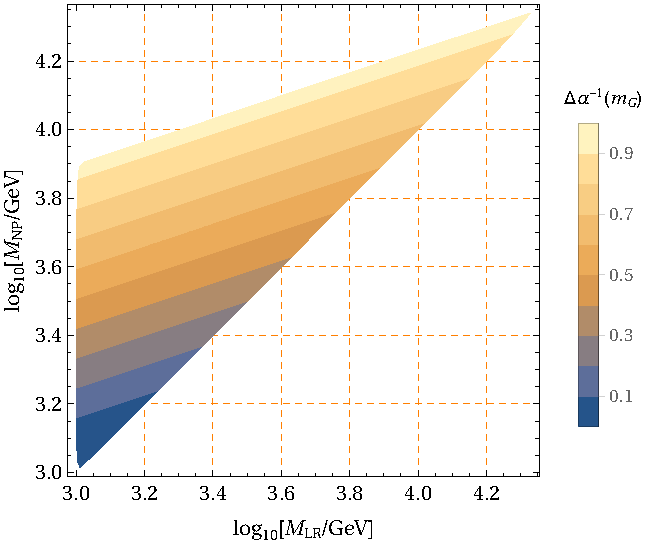
\includegraphics[width=0.43\textwidth]{ParamSpaceI}  
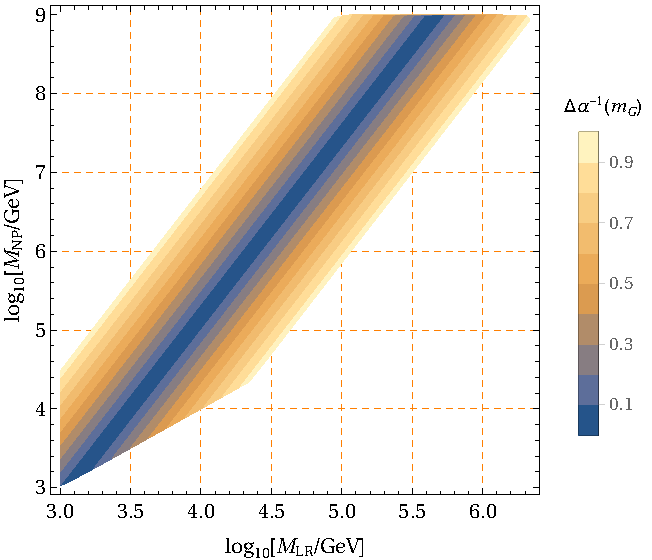
\includegraphics[width=0.42\textwidth]{ParamSpaceII} 
\end{frame}

\begin{frame}
  \frametitle{Conclusions}
  In addition to accommodate usual simplified dark matter models,  Left-right symmetric standard models have additional DM portals:

  New $\Delta_R$ portal for direct detection of left-singlet right-triplet mixed dark matter, in companion with left-singlets charged and doubly charged fermions.

Next: Search for them in compressed spectra scenarios at the LHC
%Excluidos por LEP?
\end{frame}

\plain{Thanks!}
\end{document}




TEMPLATES

1. Background image slide
%%%%%%%%%%%%%%%%%%%%%%%%%%%%%%
{
\usebackgroundtemplate{\includegraphics[width=\paperwidth]{file}}
\setbeamertemplate{blocks}[rounded][shadow=false]
\setbeamercovered{invisible}
\begin{frame}[plain]
\end{frame}
}
%%%%%%%%%%%%%%%%%%%%%%%%%%%%%%

2. Two columns
\begin{columns}
  \begin{column}{0.48\textwidth}
    
  \end{column}
  \begin{column}{0.48\textwidth}
    
  \end{column}
\end{columns}




\begin{columns}
  \column{.48\textwidth}
  \begin{block}<2->{}
  \end{block}
  \column{.48\textwidth}
  \begin{block}<2->{}
  \end{block}
\end{columns}

%%%%%%%%%%%%%%%%%%%%%
{
\usebackgroundtemplate{\includegraphics[width=\paperwidth]{file}}
\setbeamertemplate{blocks}[rounded][shadow=false]
\setbeamercovered{invisible}
\begin{frame}[plain]
  \begin{block}{}
    Name
  \end{block}
\end{frame}
}
%%%%
{
\usebackgroundtemplate{\includegraphics[width=\paperwidth]{file}}
\setbeamertemplate{blocks}[rounded][shadow=false]
\setbeamercovered{invisible}
\begin{frame}[plain]
\end{frame}
%%%%%%%%%%%%%%%%%%
}


%Trick to put stuff in specfic places of an slide:
\begin{frame}
\begin{picture}(320,250)
\put(-25,190){D.R. \emph{et al}: arXiv:1006.5075 [PRD]\qquad\qquad arXiv:1206.3605 [PRD]}
\put(-37,20){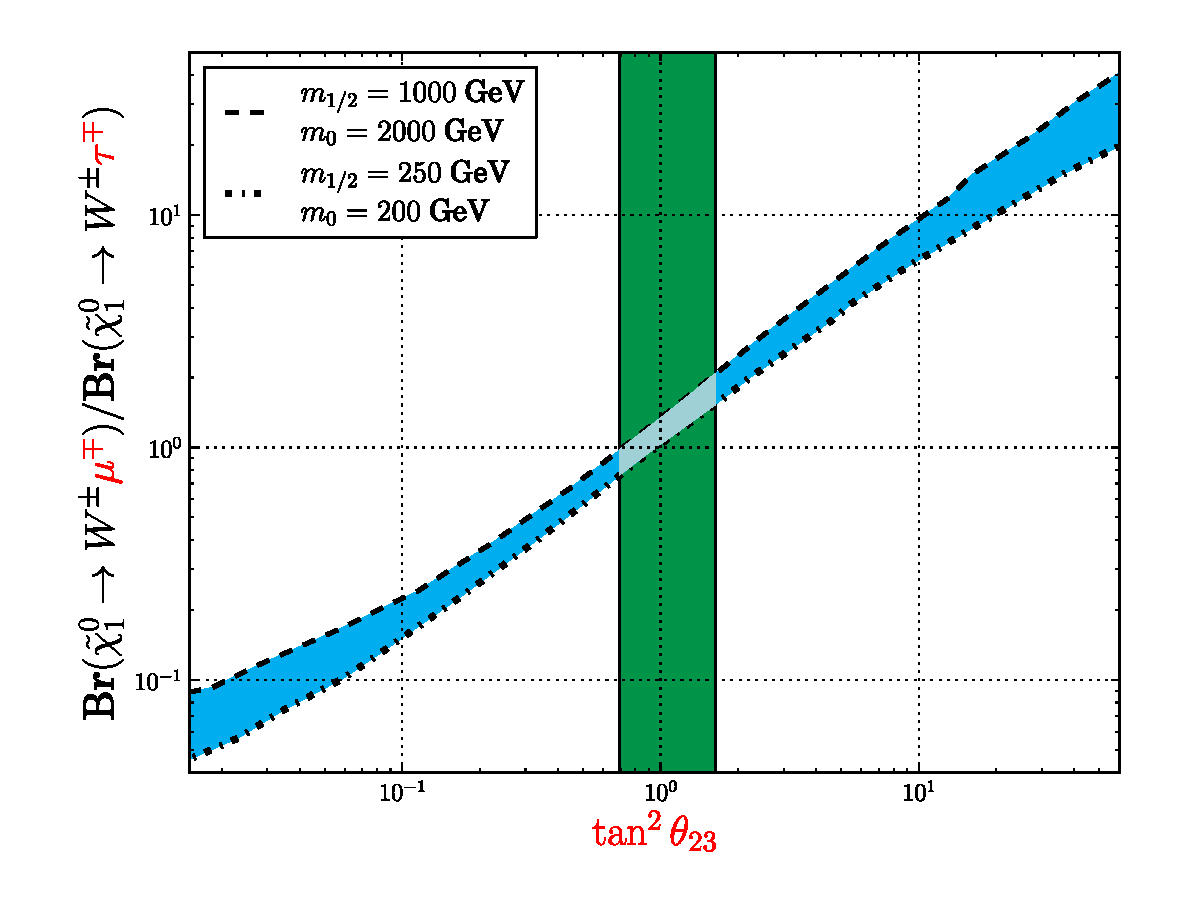
\includegraphics[scale=0.35]{atmcorrelationm}}
\put(143,20){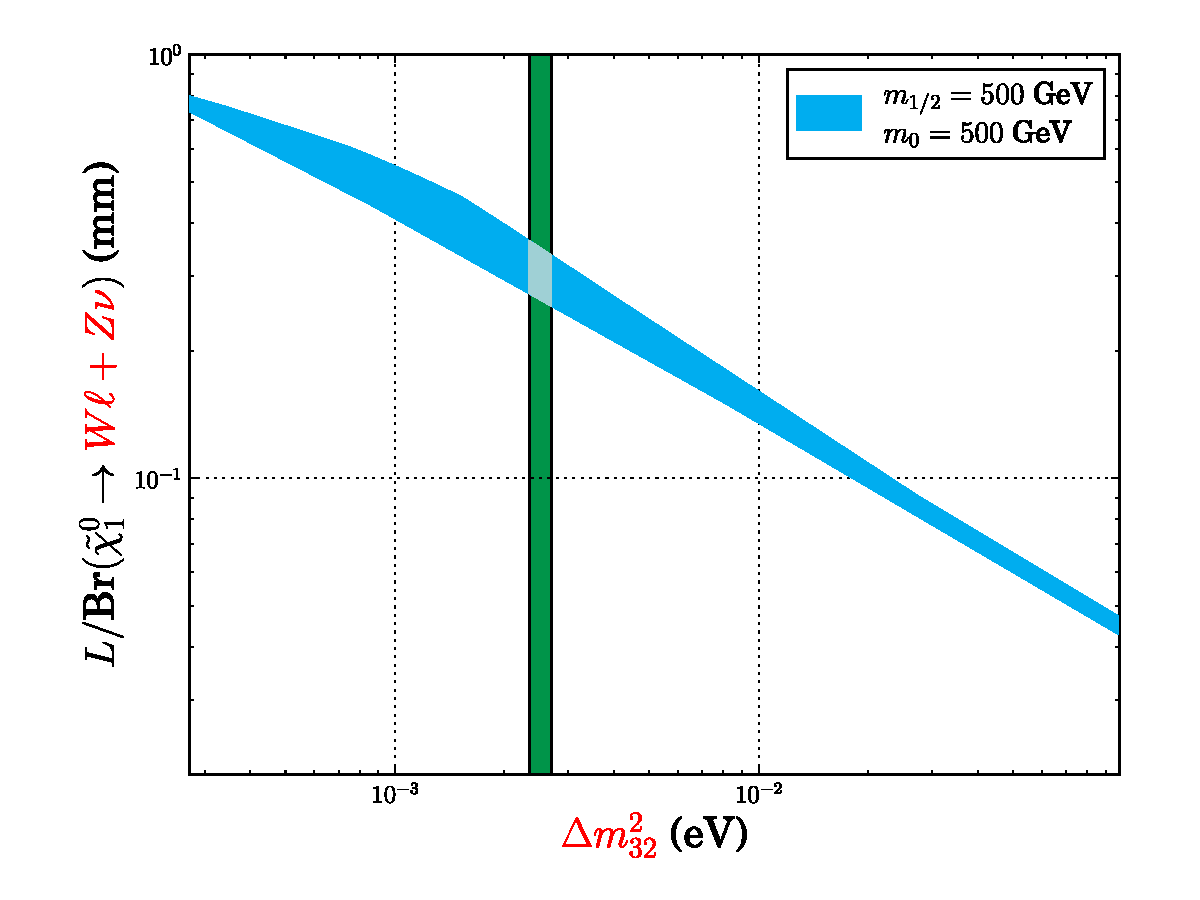
\includegraphics[scale=0.35]{LoverWlZnu_Dm23_500_500_randomm}}
\put(0,160){Only depend in \alert{$\Lambda_i$}}
\end{picture}
\end{frame}
%%%%%
Background like
%%%%%%%%%%%%%%%%%%%%%%%%
\begin{frame}[plain]
\begin{picture}(320,250)
\only<1>{\put(-30,-15){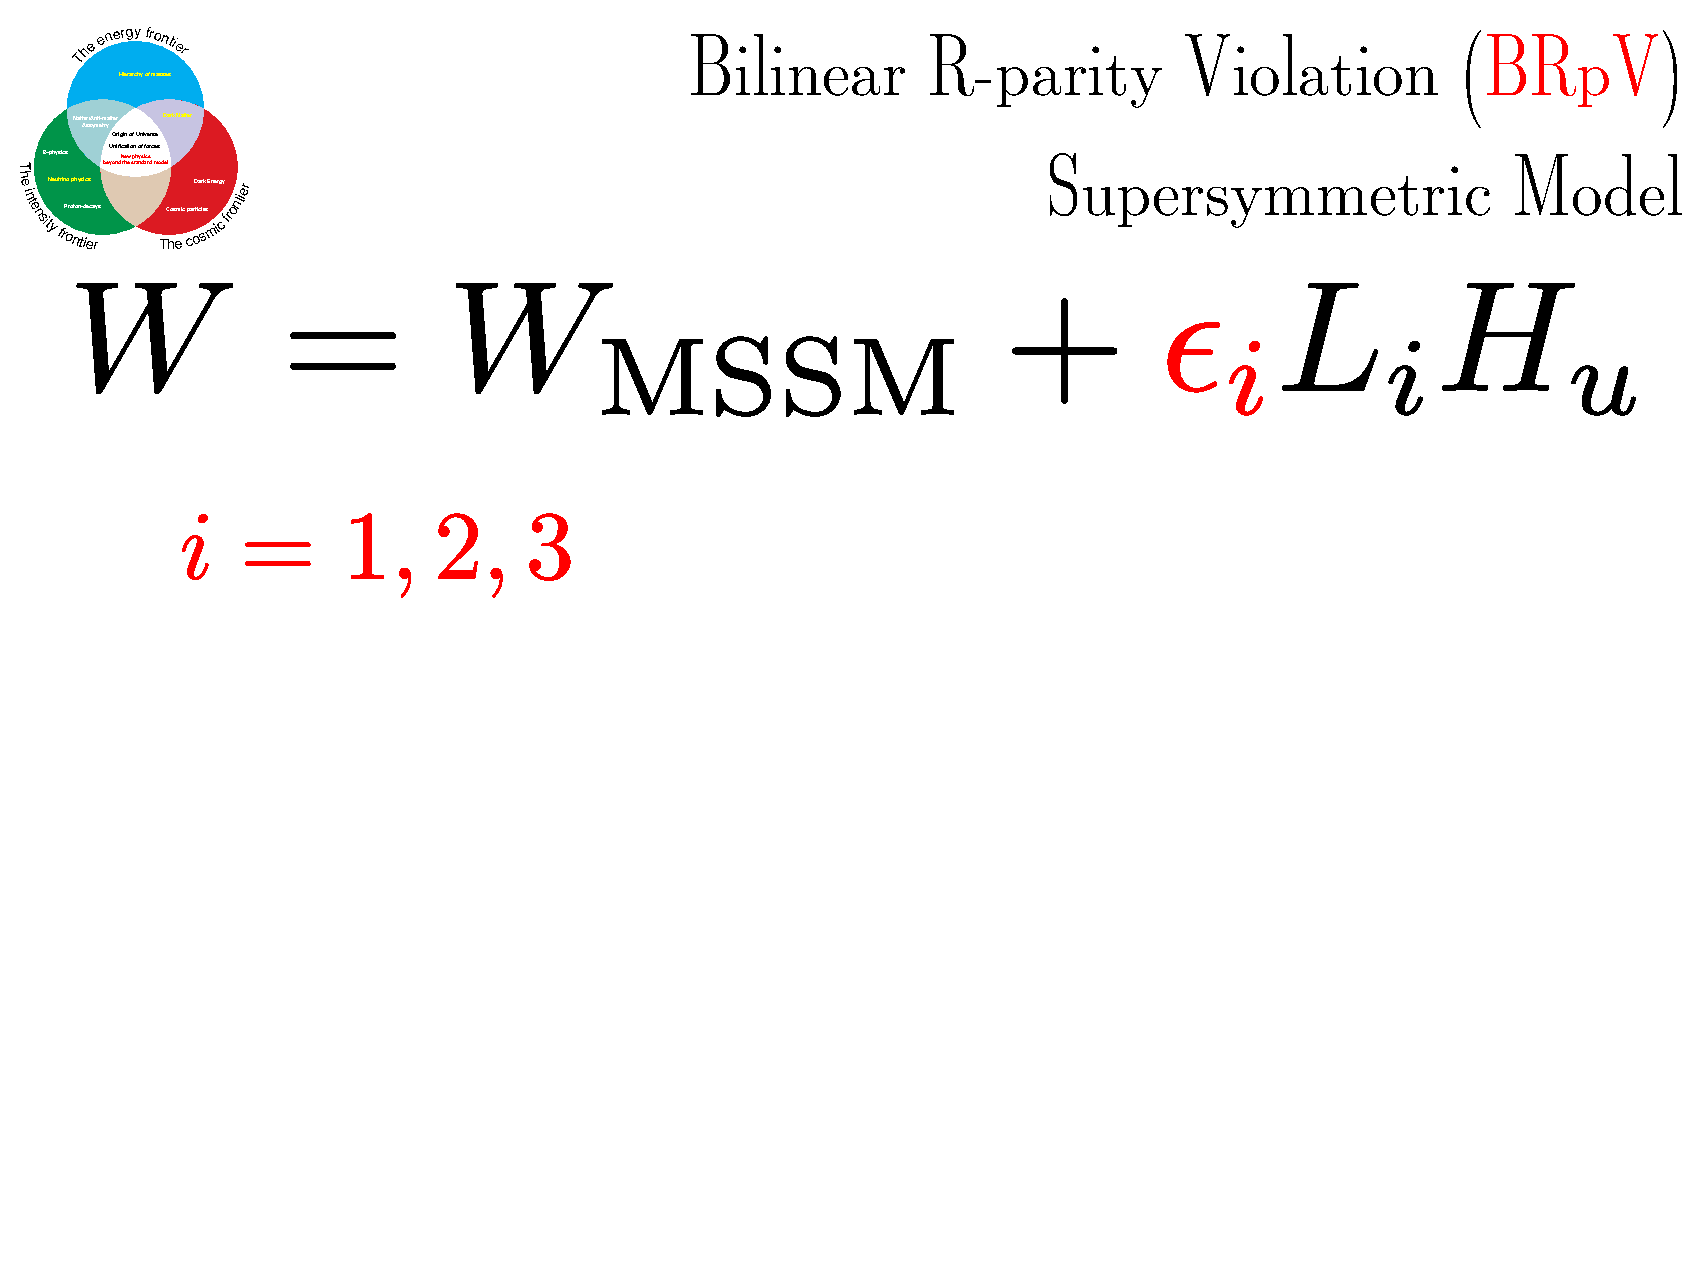
\includegraphics[width=\paperwidth]{brpv1}}}%
\only<2>{\put(-30,-15){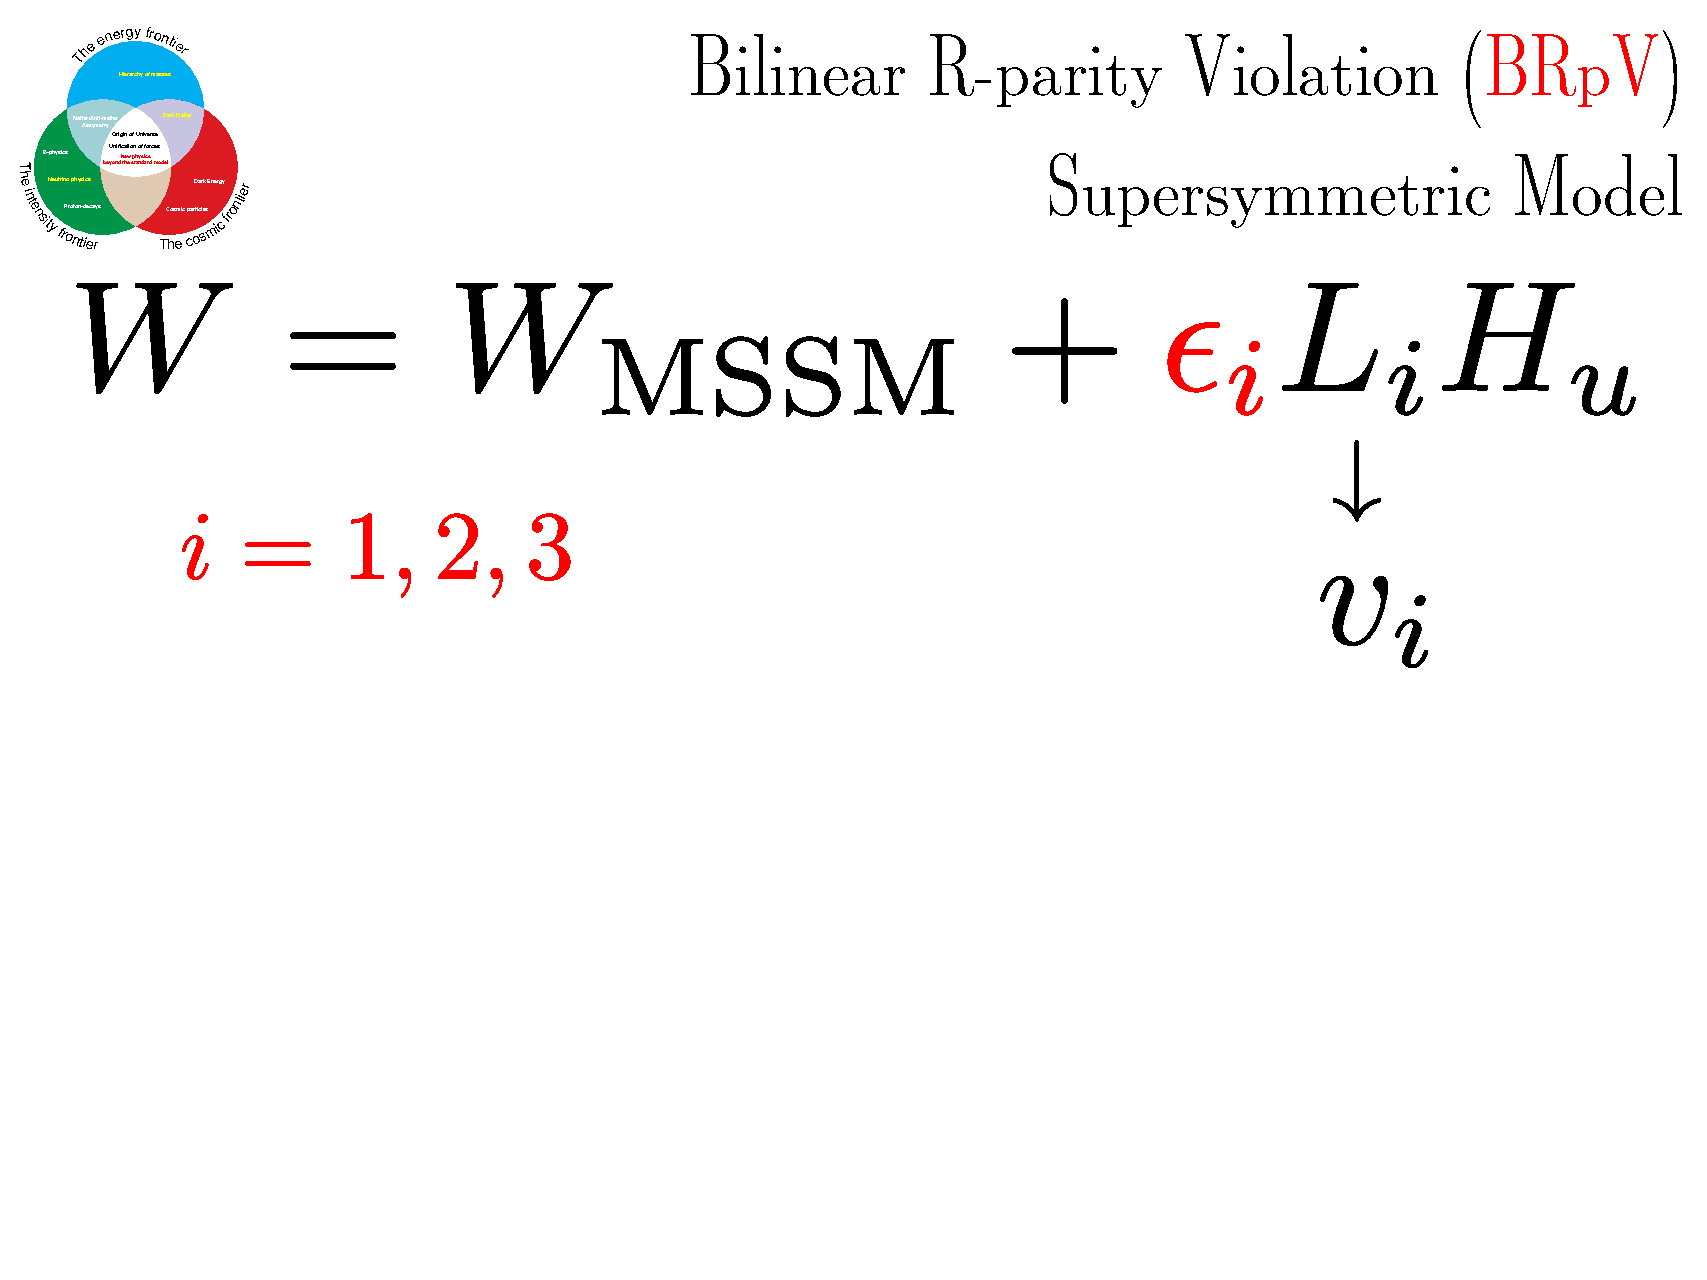
\includegraphics[width=\paperwidth]{brpv2}}}%    
\only<2>{\put(-30,-15){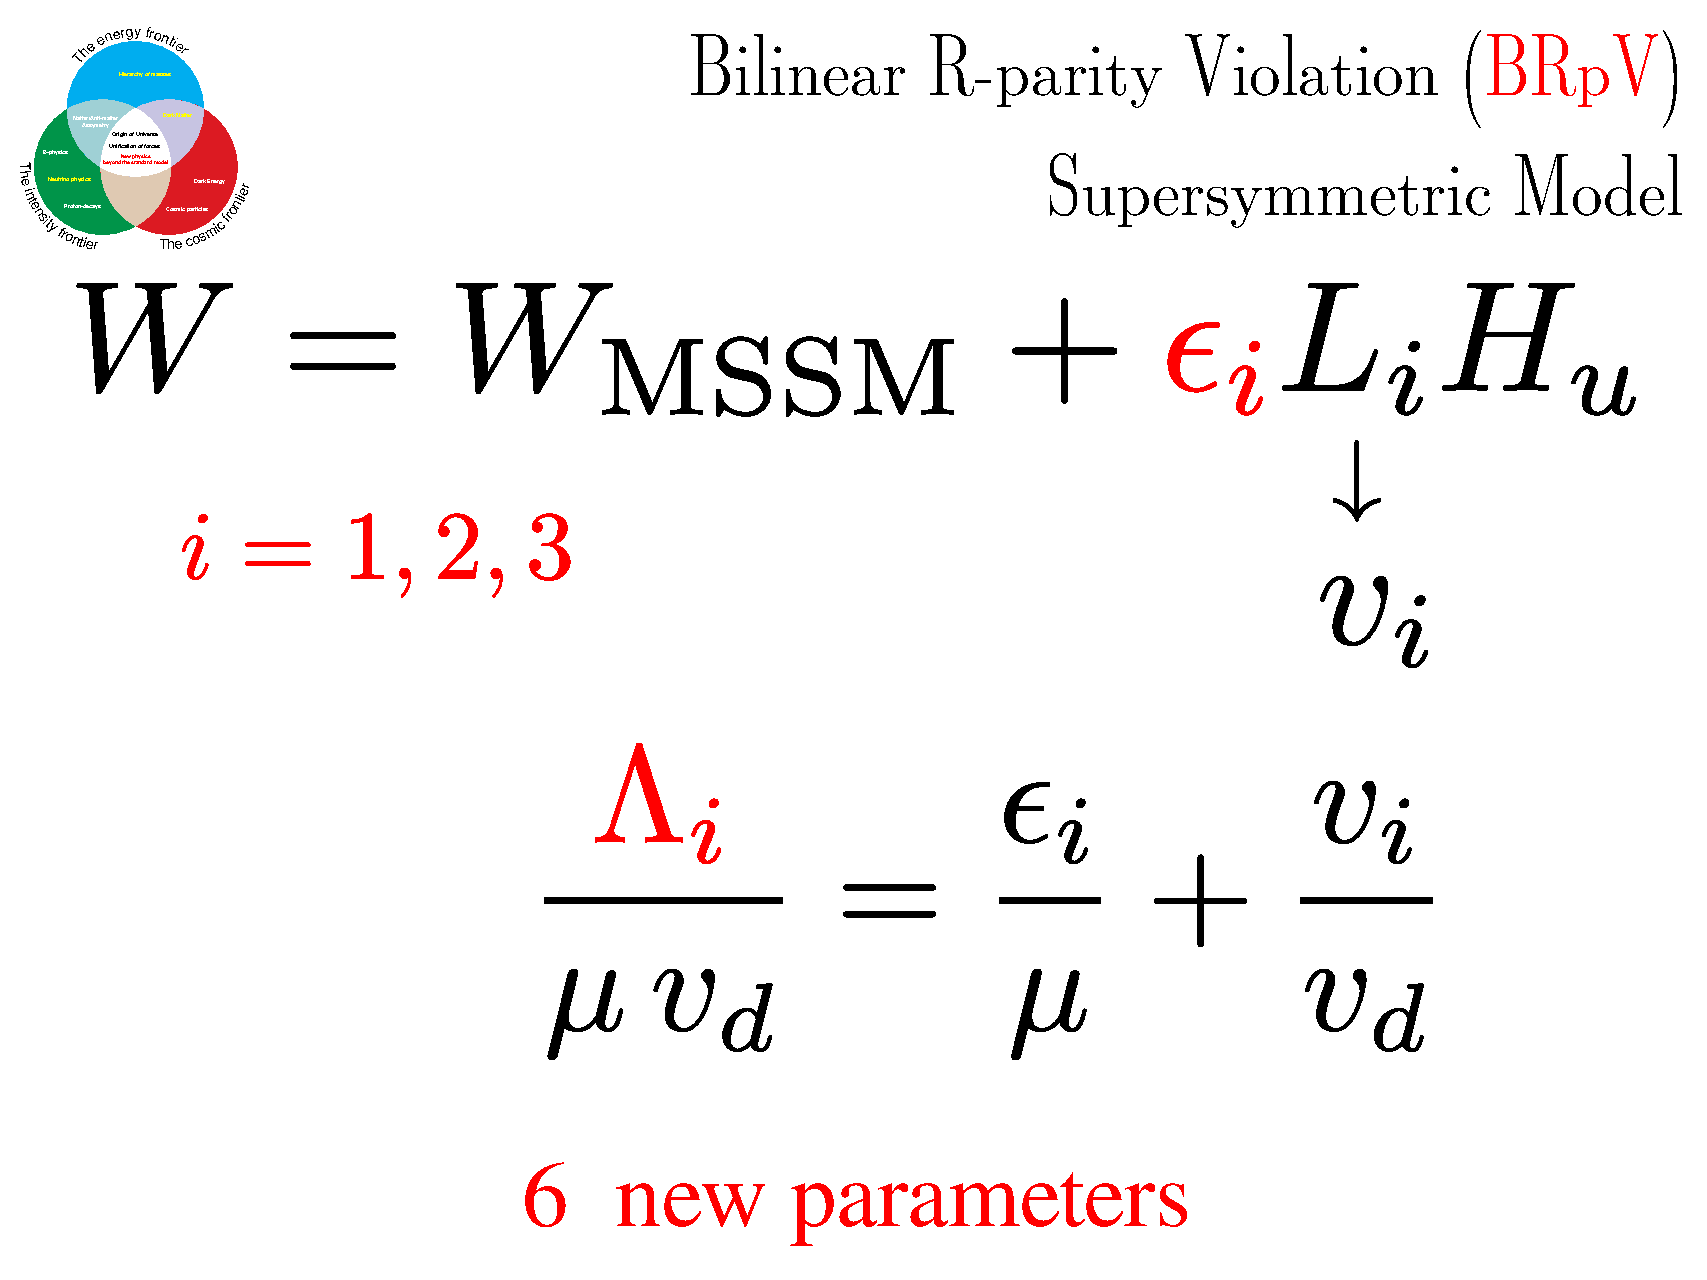
\includegraphics[width=\paperwidth]{brpv3}}}%    
\end{picture}
\end{frame}


%%%
Post it

\setbeamercolor{postit}{fg=black,bg=yellow}
\begin{beamercolorbox}[sep=1em,wd=5cm]{postit}
Place me somewhere!
\end{beamercolorbox}

%%%combine with textblock
\begin{textblock*}{297mm}(0mm,0mm)%
\begin{beamercolorbox}[sep=0.1em,wd=4cm,center,rounded=true,shadow=true]{cite}
\scriptsize Akhmedov, hep-ph/0001264
\end{beamercolorbox}
\end{textblock*}

%%More colorboxes
\setlength{\fboxrule}{3 pt}
\fcolorbox{red}{yellow}{caja de fondo
amarillo y contorno rojo}\\
\setlength{\fboxsep}{5pt}
\fcolorbox{red}{yellow}{caja de fondo
amarillo y contorno rojo}

\only<11>{\put(-20,80){
\begin{minipage}[t]{1.0\linewidth}
%\metroset{block=fill}
\begin{block}{SM particles}
     Gauge invariance+Lorentz Invariance$\to$Lagrangian (interactions)   
\end{block}
    \end{minipage}
}}


\begin{frame}
\begin{picture}(320,250)
\only<1->{\put(0,100){
  \begin{overpic}[scale=0.4,grid
            ]{table1}
\put(40,38){\tikz \draw[red,thick,rounded corners] (0,0) rectangle (2,0.5);}
  \end{overpic}
}
}
%%%circle
\end{picture}
\end{frame}
